\chapter{Quantification of Spatial Self-Shielding Effects}
\label{chap:quantify}


%%%%%%%%%%%%%%%%%%%%%%%%%%%%%%%%%%%%%%%%%%%%%%%%%%%%%%%%%%%%%%%%%%%%%%%%%%%%%%%
\section{Overview}
\label{sec:chap8-overview}

The preceding chapter introduced six heterogeneous 2D \ac{PWR} benchmarks derived from the \ac{BEAVRS} model, along with reference metrics tallied by OpenMC. This chapter applies multi-group transport calculations to model the same benchmarks in OpenMOC with \ac{MGXS} generated by OpenMC. The objective is to identify the bias between OpenMC and OpenMOC for \ac{MGXS} libraries which account for spatial self-shielding effects\footnote{The effects of neighboring pins, grid spacers, inter-assembly grid sleeves, and the core baffle, barrel and vessel are all of interest in the context of spatial self-shielding in this and subsequent chapters.} to varying degrees. In particular, this chapter quantifies the difference in the approximation error between simulations in which the same \ac{MGXS} are used in each unique fuel pin (\textit{e.g.}, each fuel enrichment) and those in which unique \ac{MGXS} are used in each and every pin. The former case does little if anything to model spatial self-shielding effects, whereas the latter case ``fully'' resolves these effects, albeit at the expense of very large \ac{MGXS} libraries. This difference in approximation error motivates the development of a novel methodology in the following chapters which use statistical clustering to capture spatial self-shielding effects in \ac{MGXS}.

Three different schemes for spatial homogenization of pin-wise \ac{MGXS} are introduced in Sec.~\ref{sec:chap8-pinwise-space-homogenize}. The discretized models and runtime parameters used in the OpenMOC simulations are detailed in Sec.~\ref{sec:chap8-moc-params}. The bias between the OpenMOC simulations and the reference OpenMC results -- including eigenvalues, pin-wise fission rates and pin-wise U-238 capture rates -- are presented in Sec.~\ref{sec:chap8-mg-results}. The need for a new, more flexible and specialized approach to spatial homogenization which appropriately captures spatial self-shielding effects with minimal computational expense is discussed in Sec.~\ref{sec:chap8-mgxs-converge}.


%%%%%%%%%%%%%%%%%%%%%%%%%%%%%%%%%%%%%%%%%%%%%%%%%%%%%%%%%%%%%%%%%%%%%%%%%%%%%%%
\section{Pin-wise Spatial Homogenization Schemes}
\label{sec:chap8-pinwise-space-homogenize}

This chapter employs three different spatial homogenization schemes to model spatial self-shielding effects in \ac{MGXS}. Although all spatial zones may experience spatial self-shielding, this chapter only models the impact of spatial self-shielding on \ac{MGXS} in fissile regions. The \textit{infinite}, \textit{null} and \textit{degenerate} spatial homogenization schemes are introduced in Secs.~\Crefrange{subsec:chap8-infinite}{subsec:chap8-degenerate}. These schemes model spatial self-shielding for each fuel pin with increasing granularity and complexity. The total number of materials (\textit{i.e.}, \ac{MGXS}) used to model each benchmark with each homogenization scheme is given in Tab.~\ref{table:chap8-num-materials}. A fuel assembly, 2$\times$2 colorset and part of the full core \ac{BEAVRS} model are color-coded by material and illustrated in Fig.~\ref{fig:chap8-homogenization-schemes} for each homogenization scheme.

The \texttt{openmc.mgxs} module (see Sec.~\ref{subsec:chap4-mgxs}) was used to compute 70-group \ac{MGXS} with OpenMC for each of the six heterogeneous benchmarks introduced in Chap.~\ref{chap:benchmarks}. The tallied \ac{MGXS} data was condensed to coarse 2-group and 8-group structures with downstream data processing as necessary. The OpenMC simulations were performed with the same runtime parameters as those used to generate the reference results (see Sec.~\ref{sec:chap7-ref-results}). In particular, 1000 batches with 10$^{6}$ particle histories per batch were simulated for each benchmark. The fission source was converged with 200 inactive batches for the full core \ac{BEAVRS} model, while 100 inactive batches were employed for the other five benchmarks (see Sec.~\ref{subsec:chap7-src-stationarity}). OpenMC's iso-in-lab feature (see Sec.~\ref{subsec:chap4-iso-in-lab}) was employed to enable consistent comparisons between OpenMC's reference results and OpenMOC's calculations with an isotropic in lab scattering source.

\begin{table}[h!]
  \centering
  \caption[Number of materials for each spatial homogenization scheme]{Number of materials modeled with unique \ac{MGXS} in each heterogeneous benchmark for each spatial homogenization scheme.}
  \small
  \label{table:chap8-num-materials}
  \vspace{6pt}
  \begin{tabular}{l r r r}
  \toprule
  \rowcolor{lightgray}
  & \multicolumn{3}{c}{\cellcolor{lightgray} \bf \# Materials} \\
  \multirow{-2}{*}{\cellcolor{lightgray} \bf Benchmark} &
  \multicolumn{1}{c}{\cellcolor{lightgray} \bf Infinite} &
  \multicolumn{1}{c}{\cellcolor{lightgray} \bf Null} &
  \multicolumn{1}{c}{\cellcolor{lightgray} \bf Degenerate} \\
  \midrule
1.6\% Assm & 8 & 8 & 271 \\
  \midrule
3.1\% Assm & 8 & 8 & 271 \\
  \midrule
3.1\% Assm w/ 20 BPs & 10 & 10 & 273  \\
  \midrule
2$\times$2 Colorset & 11 & 11 & 1,065 \\
  \midrule
2$\times$2 Colorset w/ Reflector & 11 & 11 & 1,065 \\
  \midrule
\ac{BEAVRS} Quarter Core & 15 & 15 & 13,028 \\ % 50,964
  \bottomrule
\end{tabular}
\end{table}

\begin{figure}[h!]
\centering
\begin{subfigure}{.45\textwidth}
  \centering
  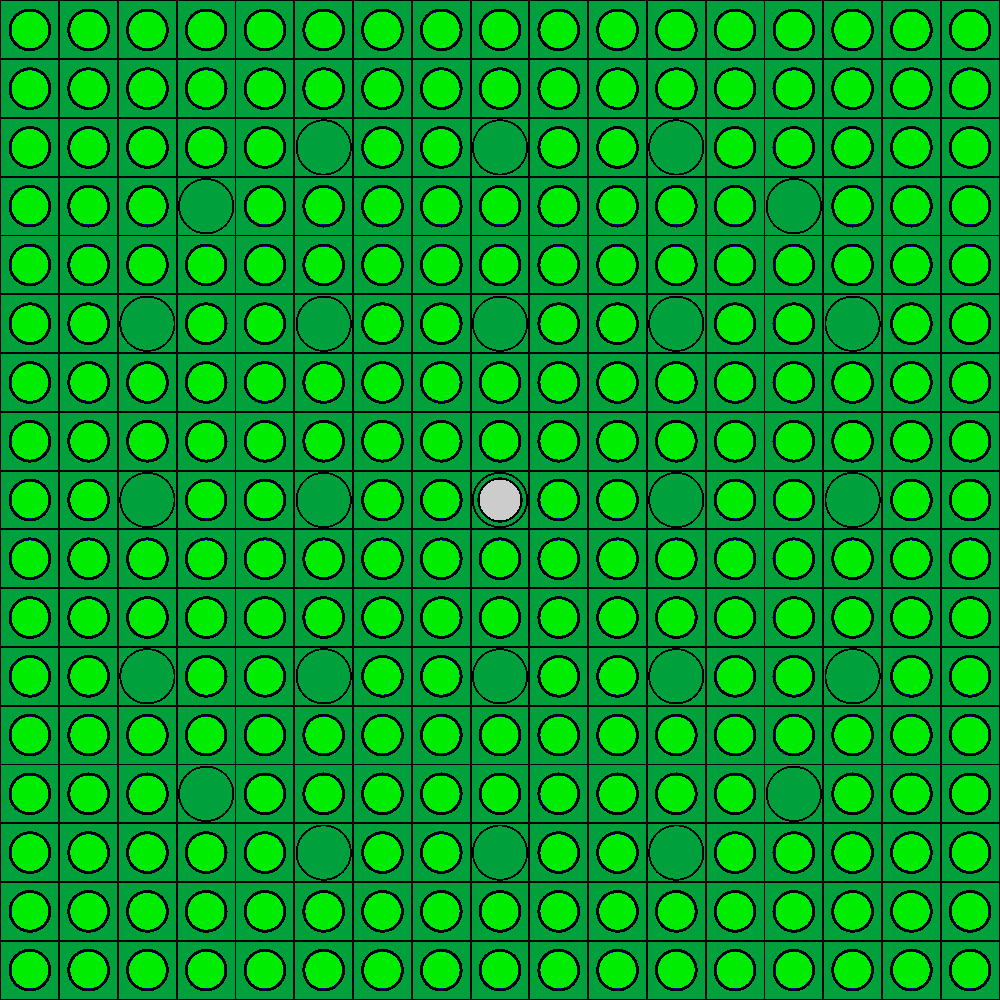
\includegraphics[width=0.87\linewidth]{figures/quantification/homogenization/assm-16-null-materials}
  \caption{}
  \label{fig:chap8-assm-16-null-materials}
\end{subfigure}%
\begin{subfigure}{.45\textwidth}
  \centering
  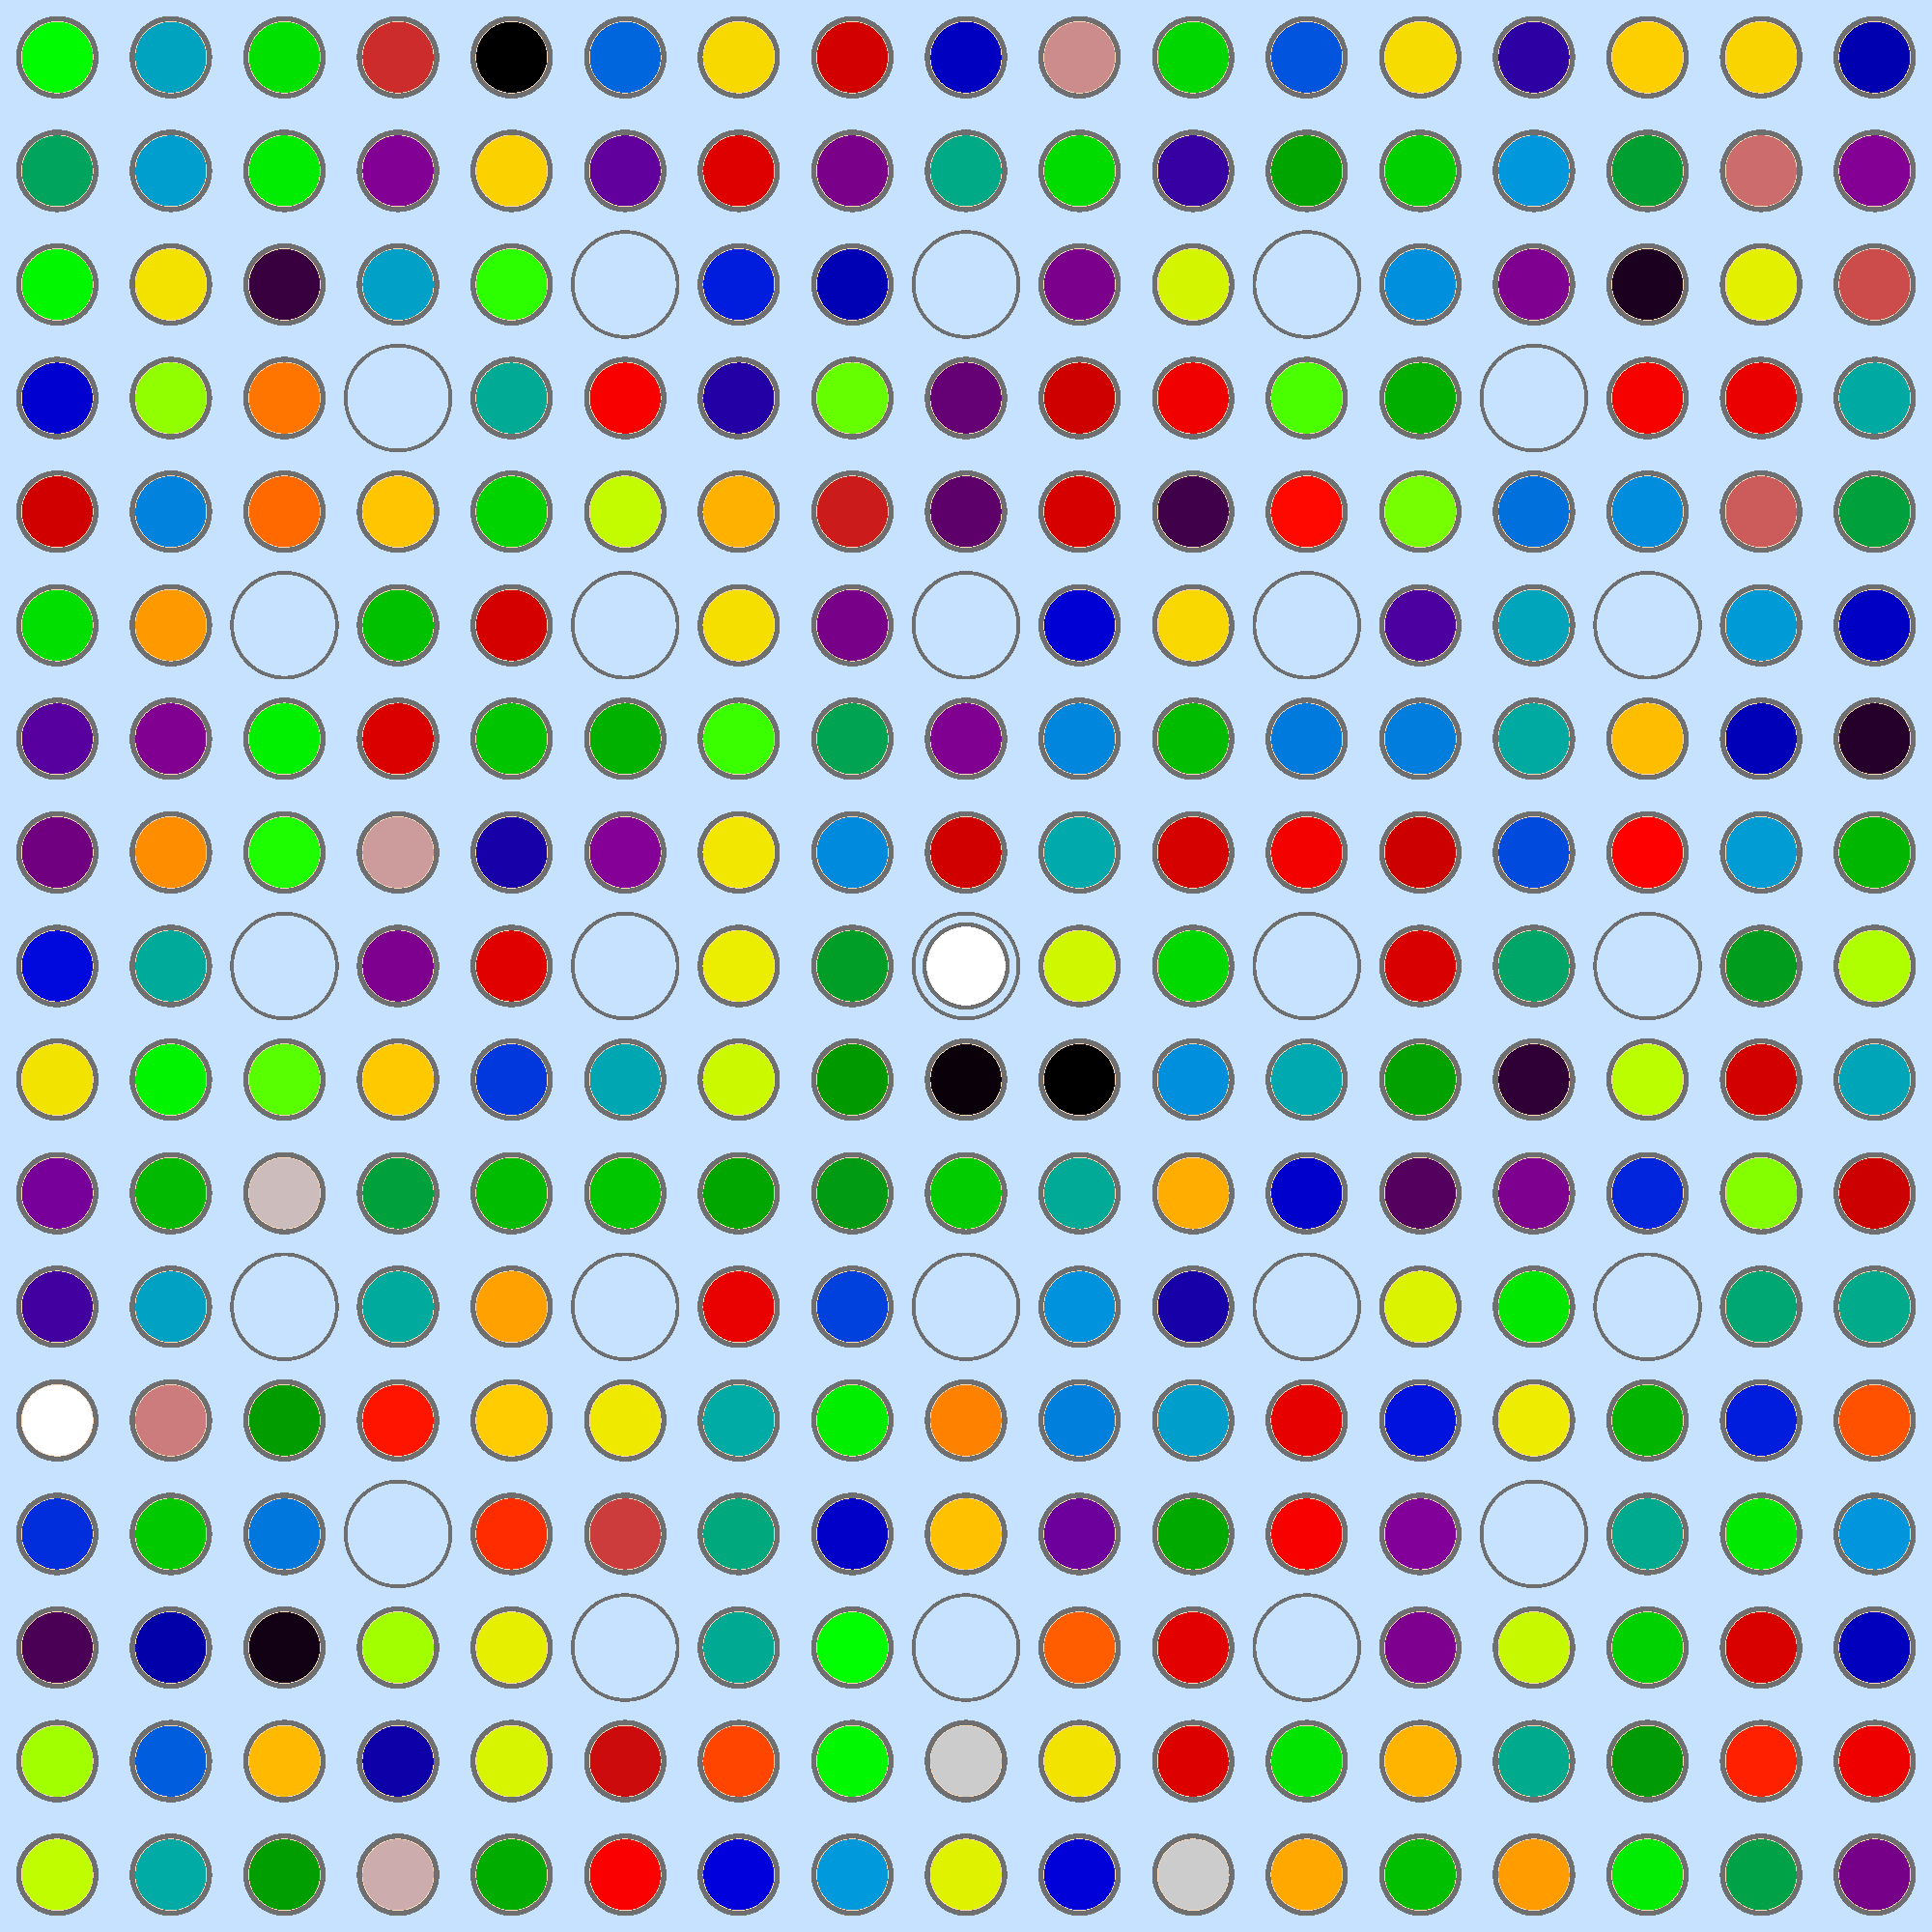
\includegraphics[width=0.87\linewidth]{figures/quantification/homogenization/assm-16-degenerate-materials}
  \caption{}
  \label{fig:chap8-assm-16-degenerate-materials}
\end{subfigure}
\begin{subfigure}{.45\textwidth}
  \centering
  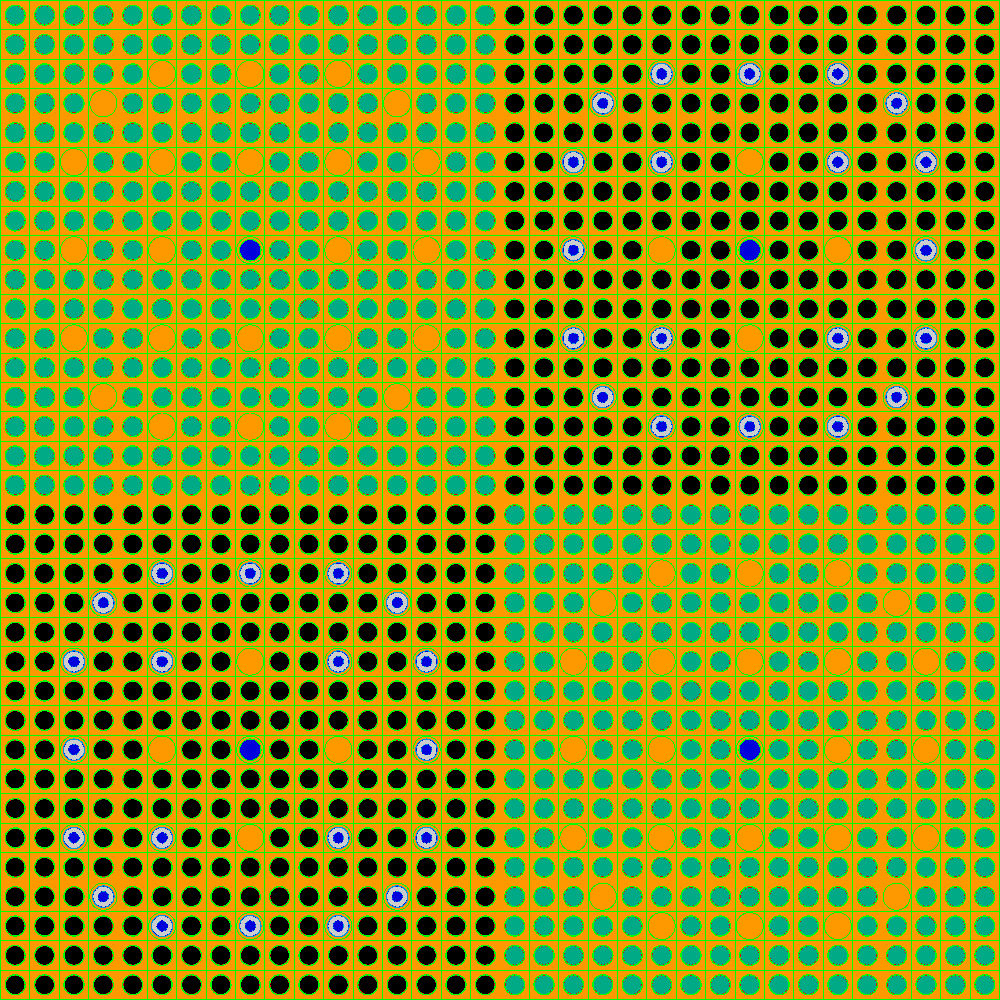
\includegraphics[width=0.87\linewidth]{figures/quantification/homogenization/2x2-null-materials}
  \caption{}
  \label{fig:chap8-2x2-null-materials}
\end{subfigure}%
\begin{subfigure}{.45\textwidth}
  \centering
  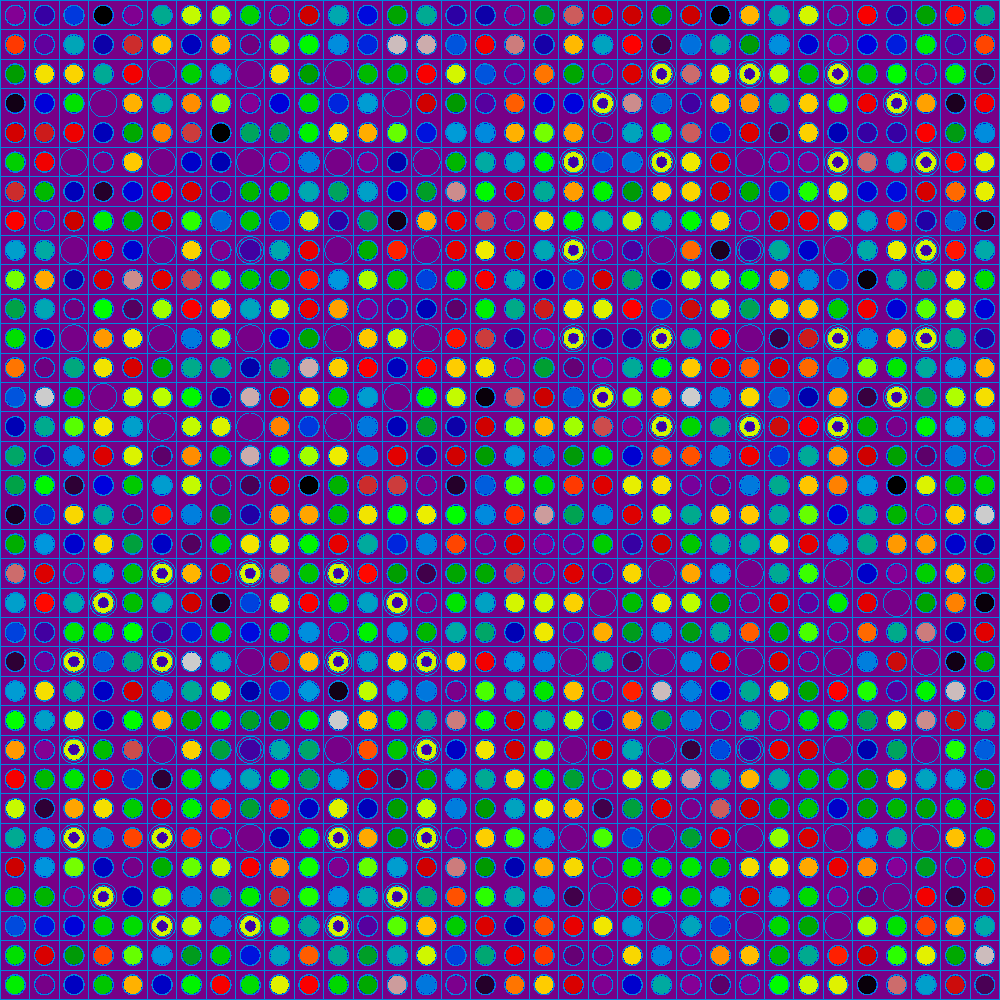
\includegraphics[width=0.87\linewidth]{figures/quantification/homogenization/2x2-degenerate-materials}
  \caption{}
  \label{fig:chap8-2x2-degenerate-materials}
\end{subfigure}
\begin{subfigure}{.45\textwidth}
  \centering
  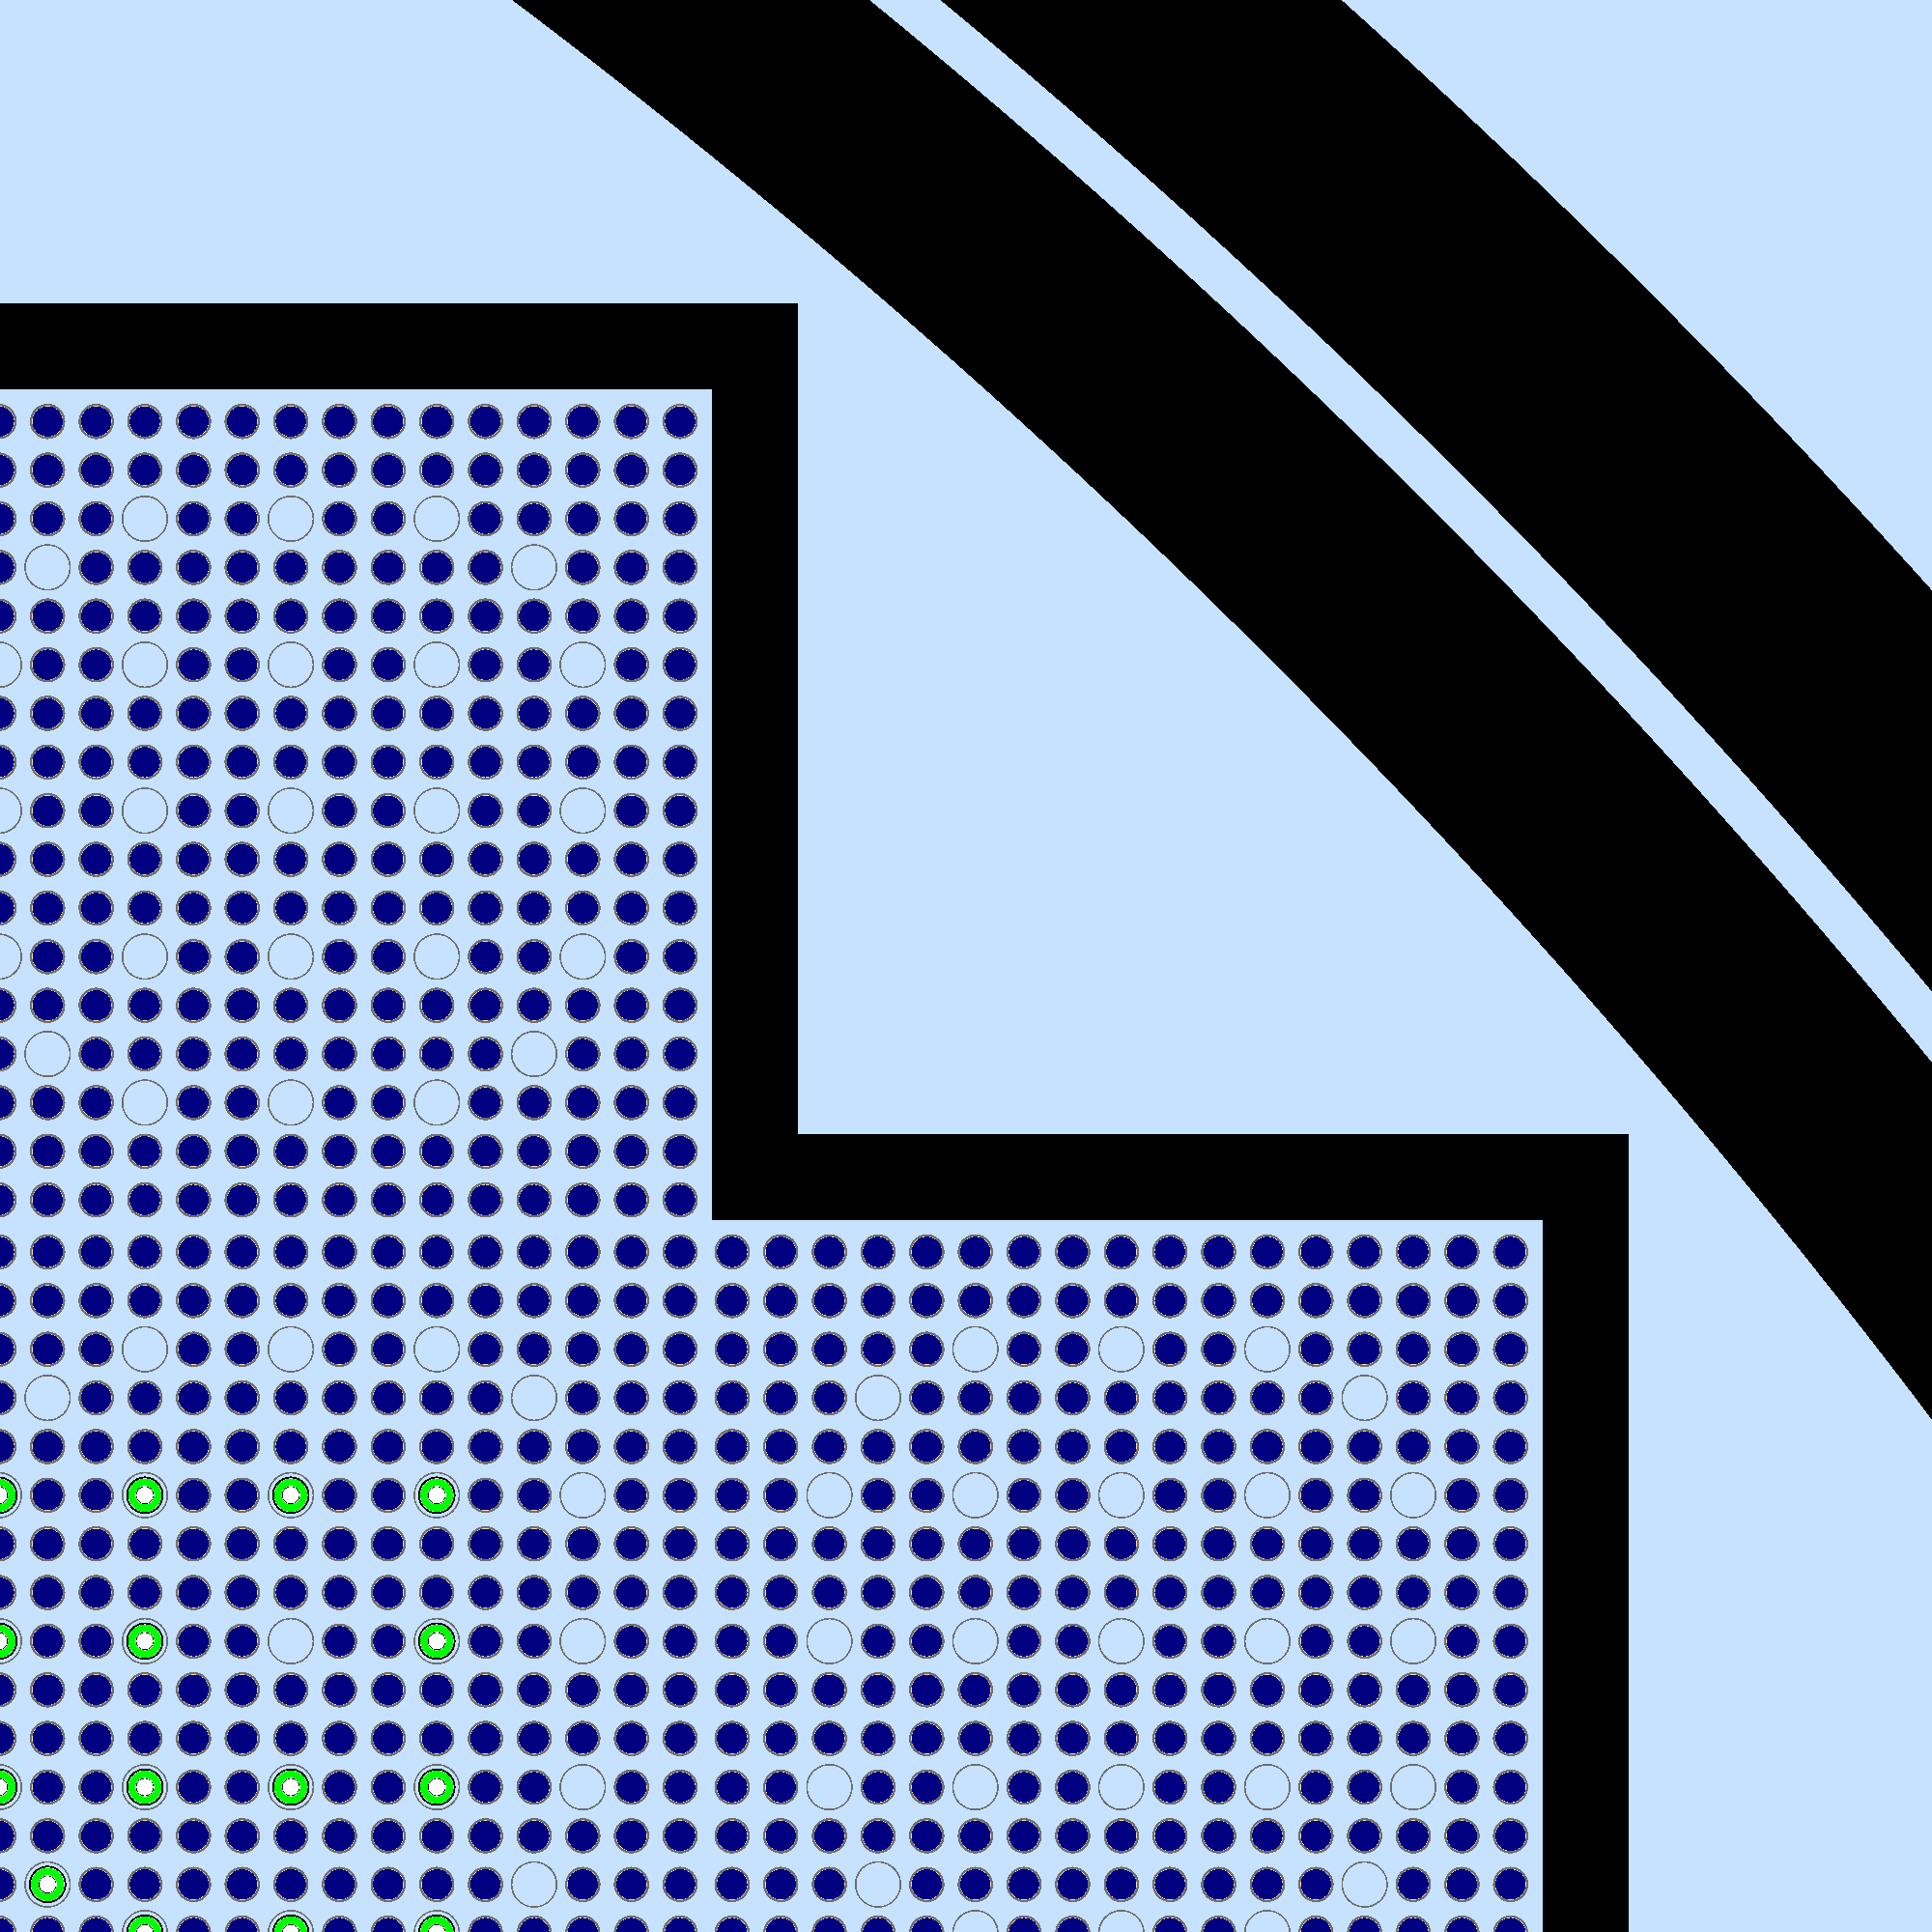
\includegraphics[width=0.87\linewidth]{figures/quantification/homogenization/full-core-null-materials}
  \caption{}
  \label{fig:chap8-full-core-null-materials}
\end{subfigure}%
\begin{subfigure}{.45\textwidth}
  \centering
  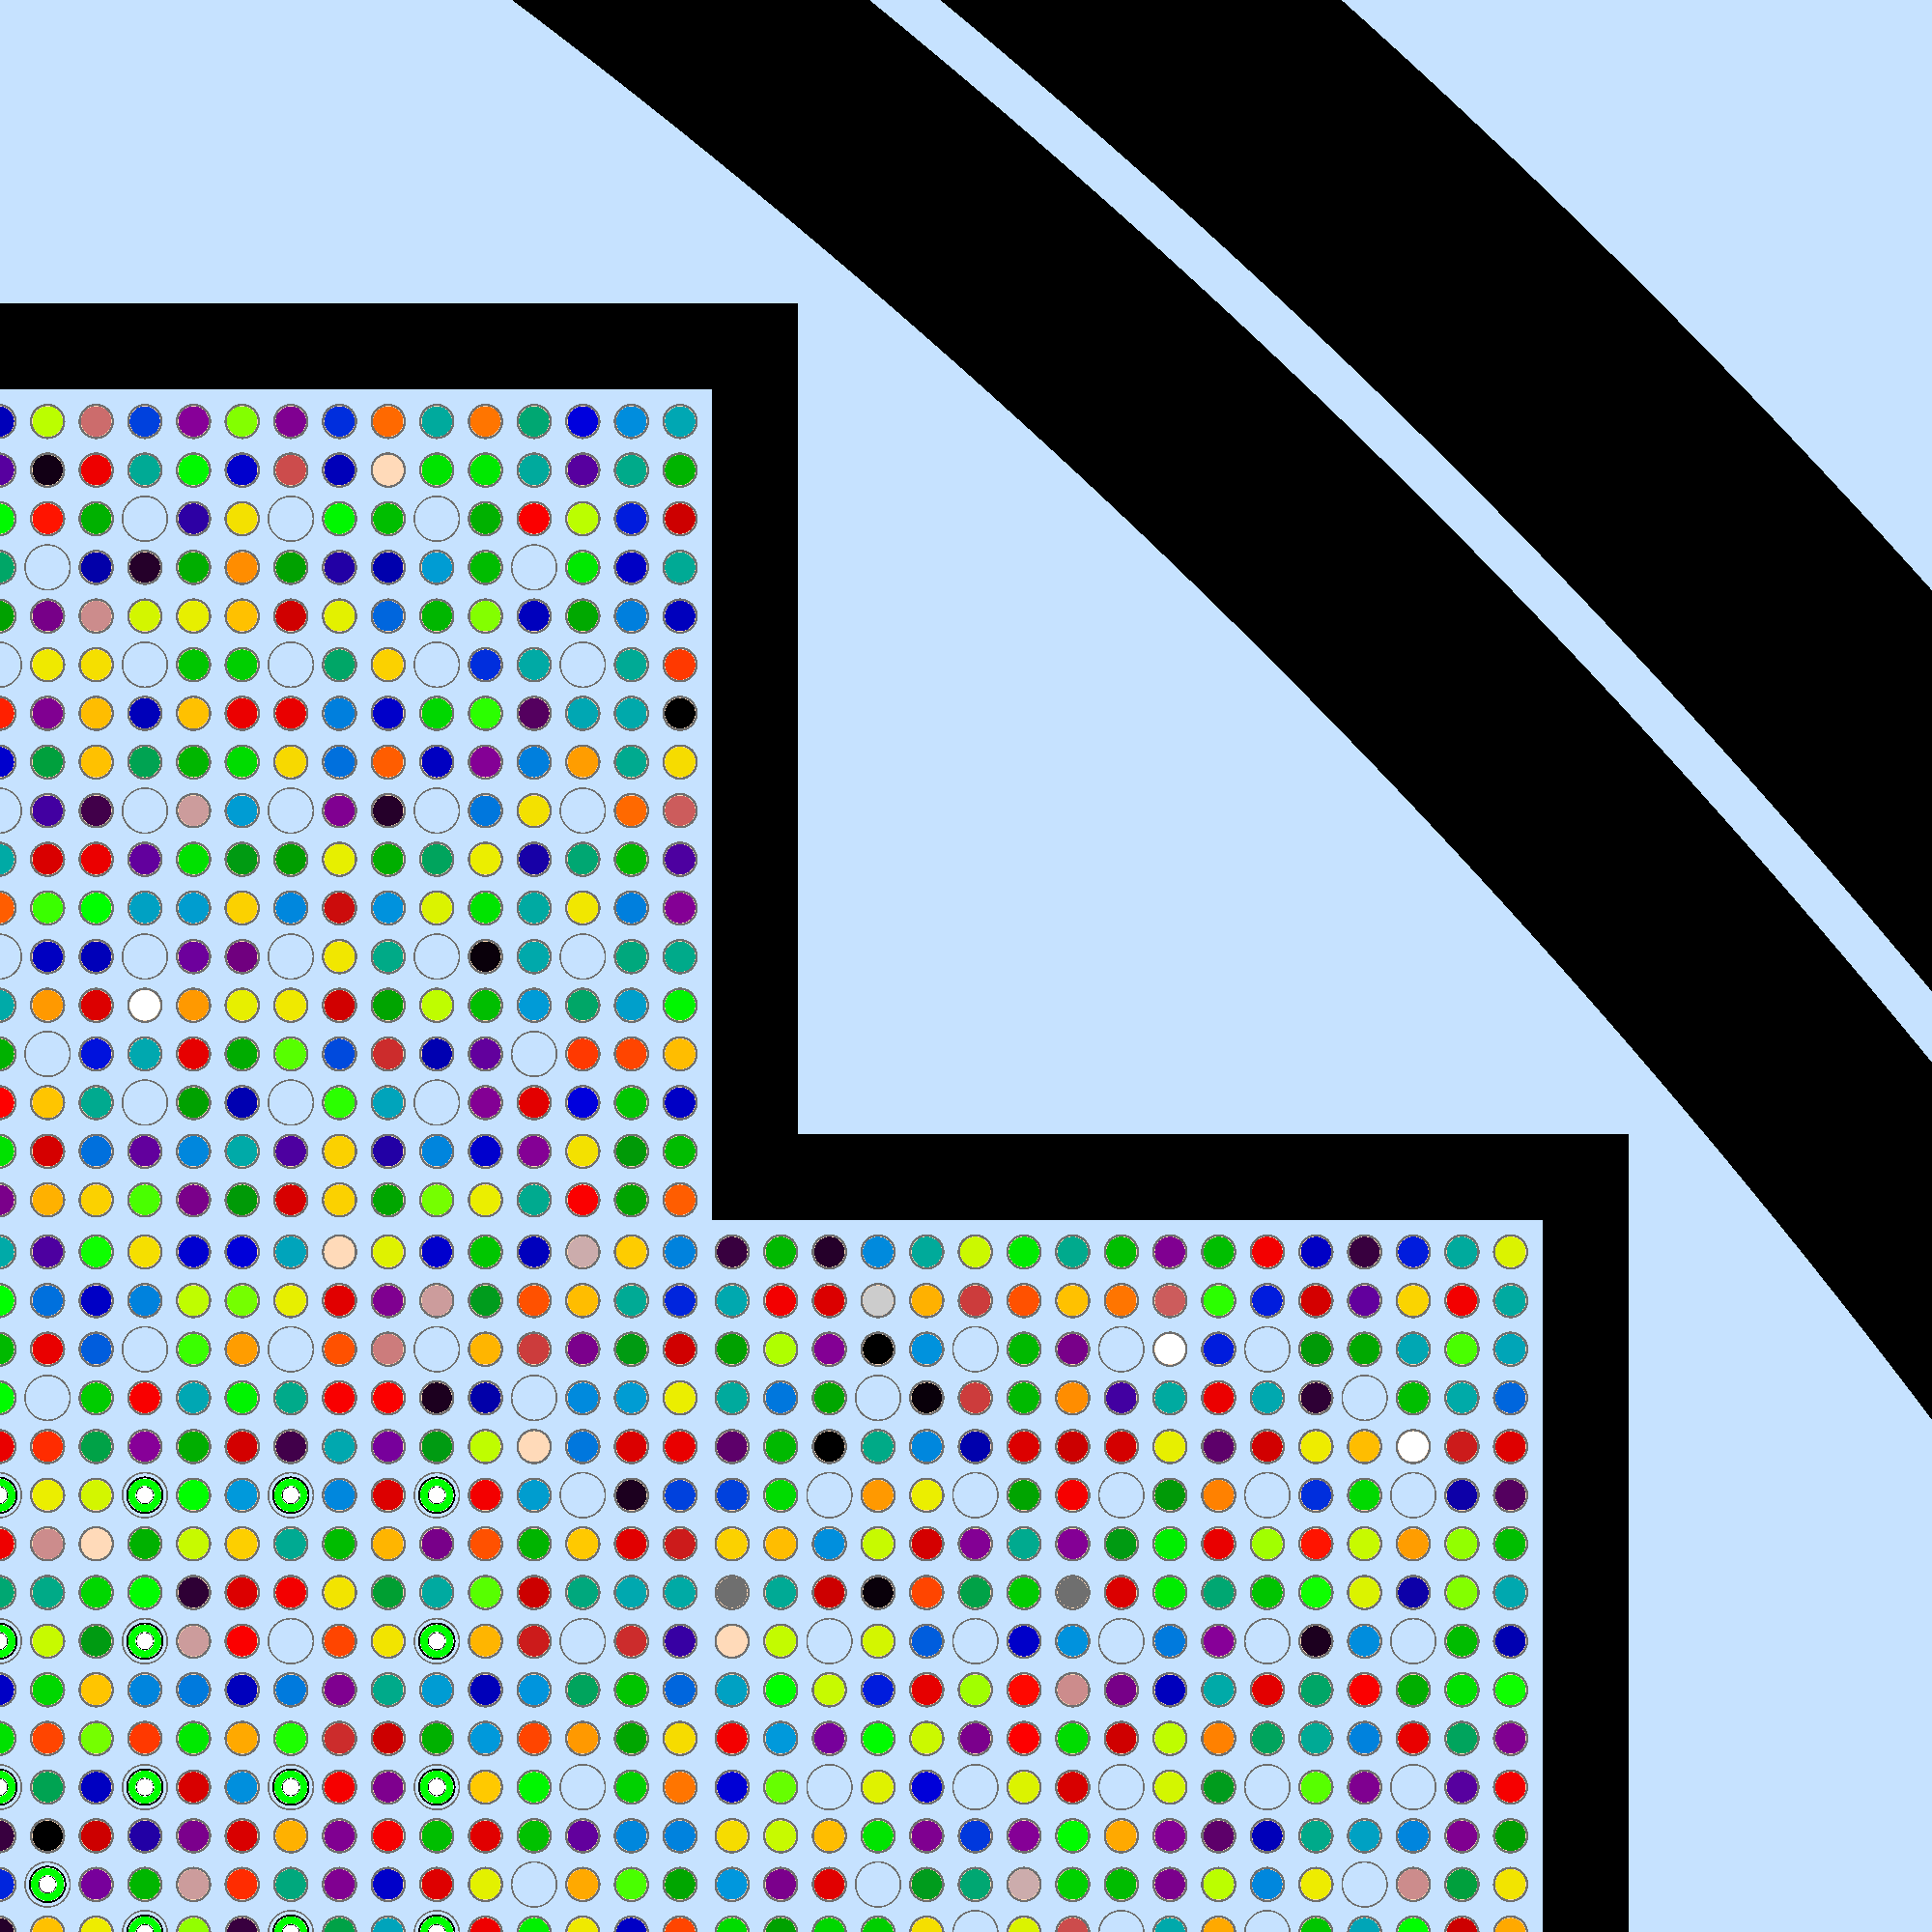
\includegraphics[width=0.87\linewidth]{figures/quantification/homogenization/full-core-degenerate-materials}
  \caption{}
  \label{fig:chap8-full-core-degenerate-materials}
\end{subfigure}
\caption[Depiction of infinite, null and degenerate spatial homogenization schemes]{OpenMOC materials for a single fuel assembly, a 2$\times$2 colorset and the 2D quarter core \ac{BEAVRS} model. The materials for the infinite and null schemes are depicted in (a), (c) and (e), and for the degenerate scheme in (b), (d) and (f), respectively. Each uniquely colored material represents a unique set of self-shielded \ac{MGXS}.}
\label{fig:chap8-homogenization-schemes}
\end{figure}

%%%%%%%%%%%%%%%%%%%%%%%%%%%%%%%%%%%%%%
\subsection{Infinite Lattice Homogenization}
\label{subsec:chap8-infinite}

The \textit{infinite} spatial homogenization scheme is most reminiscent of the traditional multi-level schemes used to generate \ac{MGXS} (see Sec.~\ref{subsec:chap2-mgxs-lib-std-approach}), and is the simplest approach to model spatial self-shielding effects considered by this thesis. The infinite scheme employs multiple OpenMC simulations to compute \ac{MGXS} for each heterogeneous benchmark. The \ac{MGXS} for each type of fuel (\textit{e.g.}, enrichment) are generated by OpenMC simulations of each fuel pin type in an infinite, repeating array\footnote{An infinite, repeating array of fuel pins is modeled by a single fuel pin with reflective boundary conditions.}. The \ac{MGXS} for all other materials -- including borated water, zircaloy, helium, etc. -- are generated from OpenMC simulations of each heterogeneous benchmark where the reaction rates and fluxes are averaged across each geometry.

The infinite scheme is designed to quantify the impact of using the ``true'' Monte Carlo flux from an infinite lattice calculation, rather than the ``true'' flux from the true heterogeneous geometry, to collapse \ac{MGXS} in fissile zones. The scheme employs a single \ac{MGXS} in each instance of a material zone, such as a fuel pin replicated many times throughout a benchmark geometry. The \ac{MGXS} for each fissile zone is generated from an infinite lattice calculation with OpenMC. The \ac{MGXS} for all non-fissile zones are generated using the ``true''  flux distribution in space and energy for each of the heterogeneous benchmarks. The scheme does not account for spatial self-shielding effects experienced by different non-fissile spatial zones filled by the same material, and instead averages these effects across the entire geometry for each material.

%-foonote: unable to run infinite pin cell calculations for non-fissile pin cells (CRGTs, BPs, instr tubes) since it's not a criticality calculation

%%%%%%%%%%%%%%%%%%%%%%%%%%%%%%%%%%%%%%
\subsection{Null Homogenization}
\label{subsec:chap8-null}

The \textit{null} spatial homogenization scheme builds upon the infinite scheme, but uses the ``true'' heterogeneous flux to collapse \ac{MGXS} for fissile as well as non-fissile materials. The null scheme eliminates the infinite lattice calculation to generate \ac{MGXS} for fissile zones, and instead uses a single Monte Carlo calculation of the complete heterogeneous geometry to generate \ac{MGXS} for \textit{all} materials. In this way, the null scheme fully abandons the multi-level approach used by the infinite scheme and most traditional approaches to generate \ac{MGXS}. Unlike the infinite scheme, the spatially self-shielded flux is used to collapse the cross sections in the fuel. However, the null scheme does not account for spatial self-shielding effects experienced by different fuel pins filled by the same type of fuel, and instead averages these effects across the entire geometry. As with the infinite scheme, a single \ac{MGXS} is employed in each instance of a material zone, such as a fuel pin replicated many times throughout a benchmark geometry.

%%%%%%%%%%%%%%%%%%%%%%%%%%%%%%%%%%%%%%
\subsection{Degenerate Homogenization}
\label{subsec:chap8-degenerate}

Unlike the infinite and null spatial homogenization schemes, the \textit{degenerate} scheme accounts for the different spatial self-shielding effects experienced by each instance of each fuel pin throughout a heterogeneous geometry. Like the null scheme, a single \ac{MC} calculation of the complete heterogeneous geometry is used to generate \ac{MGXS} for all materials. Unlike the null scheme, the \ac{MGXS} are tallied separately for each instance of fissile material zones. For example, if a heterogeneous benchmark includes $N$ fuel pins, then $N$ collections of \ac{MGXS} are separately tabulated for each fuel pin instance. The degenerate scheme tallies different \ac{MGXS} even if the isotopic compositions in the fuel pin instances are identical (\textit{e.g.}, fresh fuel at the beginning of life) since each instance may experience different spatial self-shielding effects and hence have different \ac{MGXS}.

Multi-group transport calculations with \ac{MGXS} generated using infinite/null and degenerate schemes may be compared to quantify the impact of modeling spatial self-shielding effects in \ac{MGXS} for fissile zones in heterogeneous geometries. The degenerate scheme applies the finest granularity to pin-wise spatial homogenization of any of the schemes considered in this thesis since it best captures different spatial self-shielding effects in each fuel pin. As a result, the degenerate scheme is used to benchmark the efficacy of the new methodology for spatial homogenization based on statistical clustering developed in the following chapters. Like both the infinite and null schemes, the spatial self-shielding effects experienced by different non-fissile spatial zones are averaged across the entire geometry for each non-fissile material.

The degenerate scheme generates \ac{MGXS} for each fuel pin instance using OpenMC's distributed cell tallies (see Sec.~\ref{subsec:chap4-distribcells}). The OpenCG region differentiation algorithm (see Sec.~\ref{sec:chap4-region-diff}) is used to build a new OpenMOC geometry with unique cells and materials for each fuel pin. The \ac{MGXS} are appropriately selected from OpenMC's distributed cell tallies to populate the \ac{MGXS} in the OpenMOC materials.

-need summary box for this section


%%%%%%%%%%%%%%%%%%%%%%%%%%%%%%%%%%%%%%%%%%%%%%%%%%%%%%%%%%%%%%%%%%%%%%%%%%%%%%%
\section{\ac{MOC} Runtime Parameters}
\label{sec:chap8-moc-params}

first paragraph: overview/outline
-used double precision installation of OpenMOC on INL's Falcon machine
-outline each subsection

\begin{table}[h!]
  \centering
  \caption[Number of \ac{FSR}s, tracks and segments for each heterogeneous benchmark]{Number of \ac{FSR}s, tracks and segments modeled in OpenMOC simulations of each heterogeneous benchmark.}
  \small
  \label{table:chap8-num-fsrs-tracks-segments}
  \vspace{6pt}
  \begin{tabular}{l r r r}
  \toprule
  \rowcolor{lightgray}
  \textbf{Benchmark} &
  \multicolumn{1}{c}{\cellcolor{lightgray} \textbf{\# \ac{FSR}s}} &
  \multicolumn{1}{c}{\cellcolor{lightgray} \textbf{\# Tracks}} &
  \multicolumn{1}{c}{\cellcolor{lightgray} \textbf{\# Segments}} \\
  \midrule
1.6\% Assm & 31,844 & 34,976 & 8,741,824 \\
  \midrule
3.1\% Assm & 31,844 & 34,976 & 8,741,824 \\
  \midrule
3.1\% Assm w/ 20 BPs & 32,964 & 34,976 & 8,906,064  \\
  \midrule
2$\times$2 Colorset & 188,128 & 69,892 & 44,477,312 \\
  \midrule
2$\times$2 Colorset w/ Reflector & 276,052 & 104,788 & 63,891,381 \\
  \midrule
\ac{BEAVRS} Quarter Core & 2,512,384 & 201,620 & 427,683,579 \\
  \bottomrule
\end{tabular}
\end{table}


%%%%%%%%%%%%%%%%%%%%%%%%%%%%%%%%%%%%
\subsection{Angular Discretization}
\label{subsec:chap8-angular-discretizations}

first paragraph: 
-0.05 cm track spacing
-128 azimuthal angles
-size of each track file in GB??

%%%%%%%%%%%%%%%%%%%%%%%%%%%%%%%%%%%%
\subsection{\ac{FSR} Discretization}
\label{subsec:chap8-fsr-discretizations}

first paragraph: pin cells
-Fig.~\ref{fig:chap8-pin-cell-fsrs}
-8 sectors everywhere, including the grid spacers
-num rings in fuel, moderator, guide tubes, instr tubes, BPs
-note that rings in moderator are equal spacing???
-equal volume rings in fuel, guide tube, BP

second paragraph: fuel assemblies, colorsets, full core
-Fig.~\ref{fig:chap8-pin-cell-fsrs}
-same discretization of each pin cell
-composed in each of the assembly, colorsets benchmarks introduced in preceding chapter

\begin{figure}[h!]
\centering
\begin{subfigure}{.5\textwidth}
  \centering
  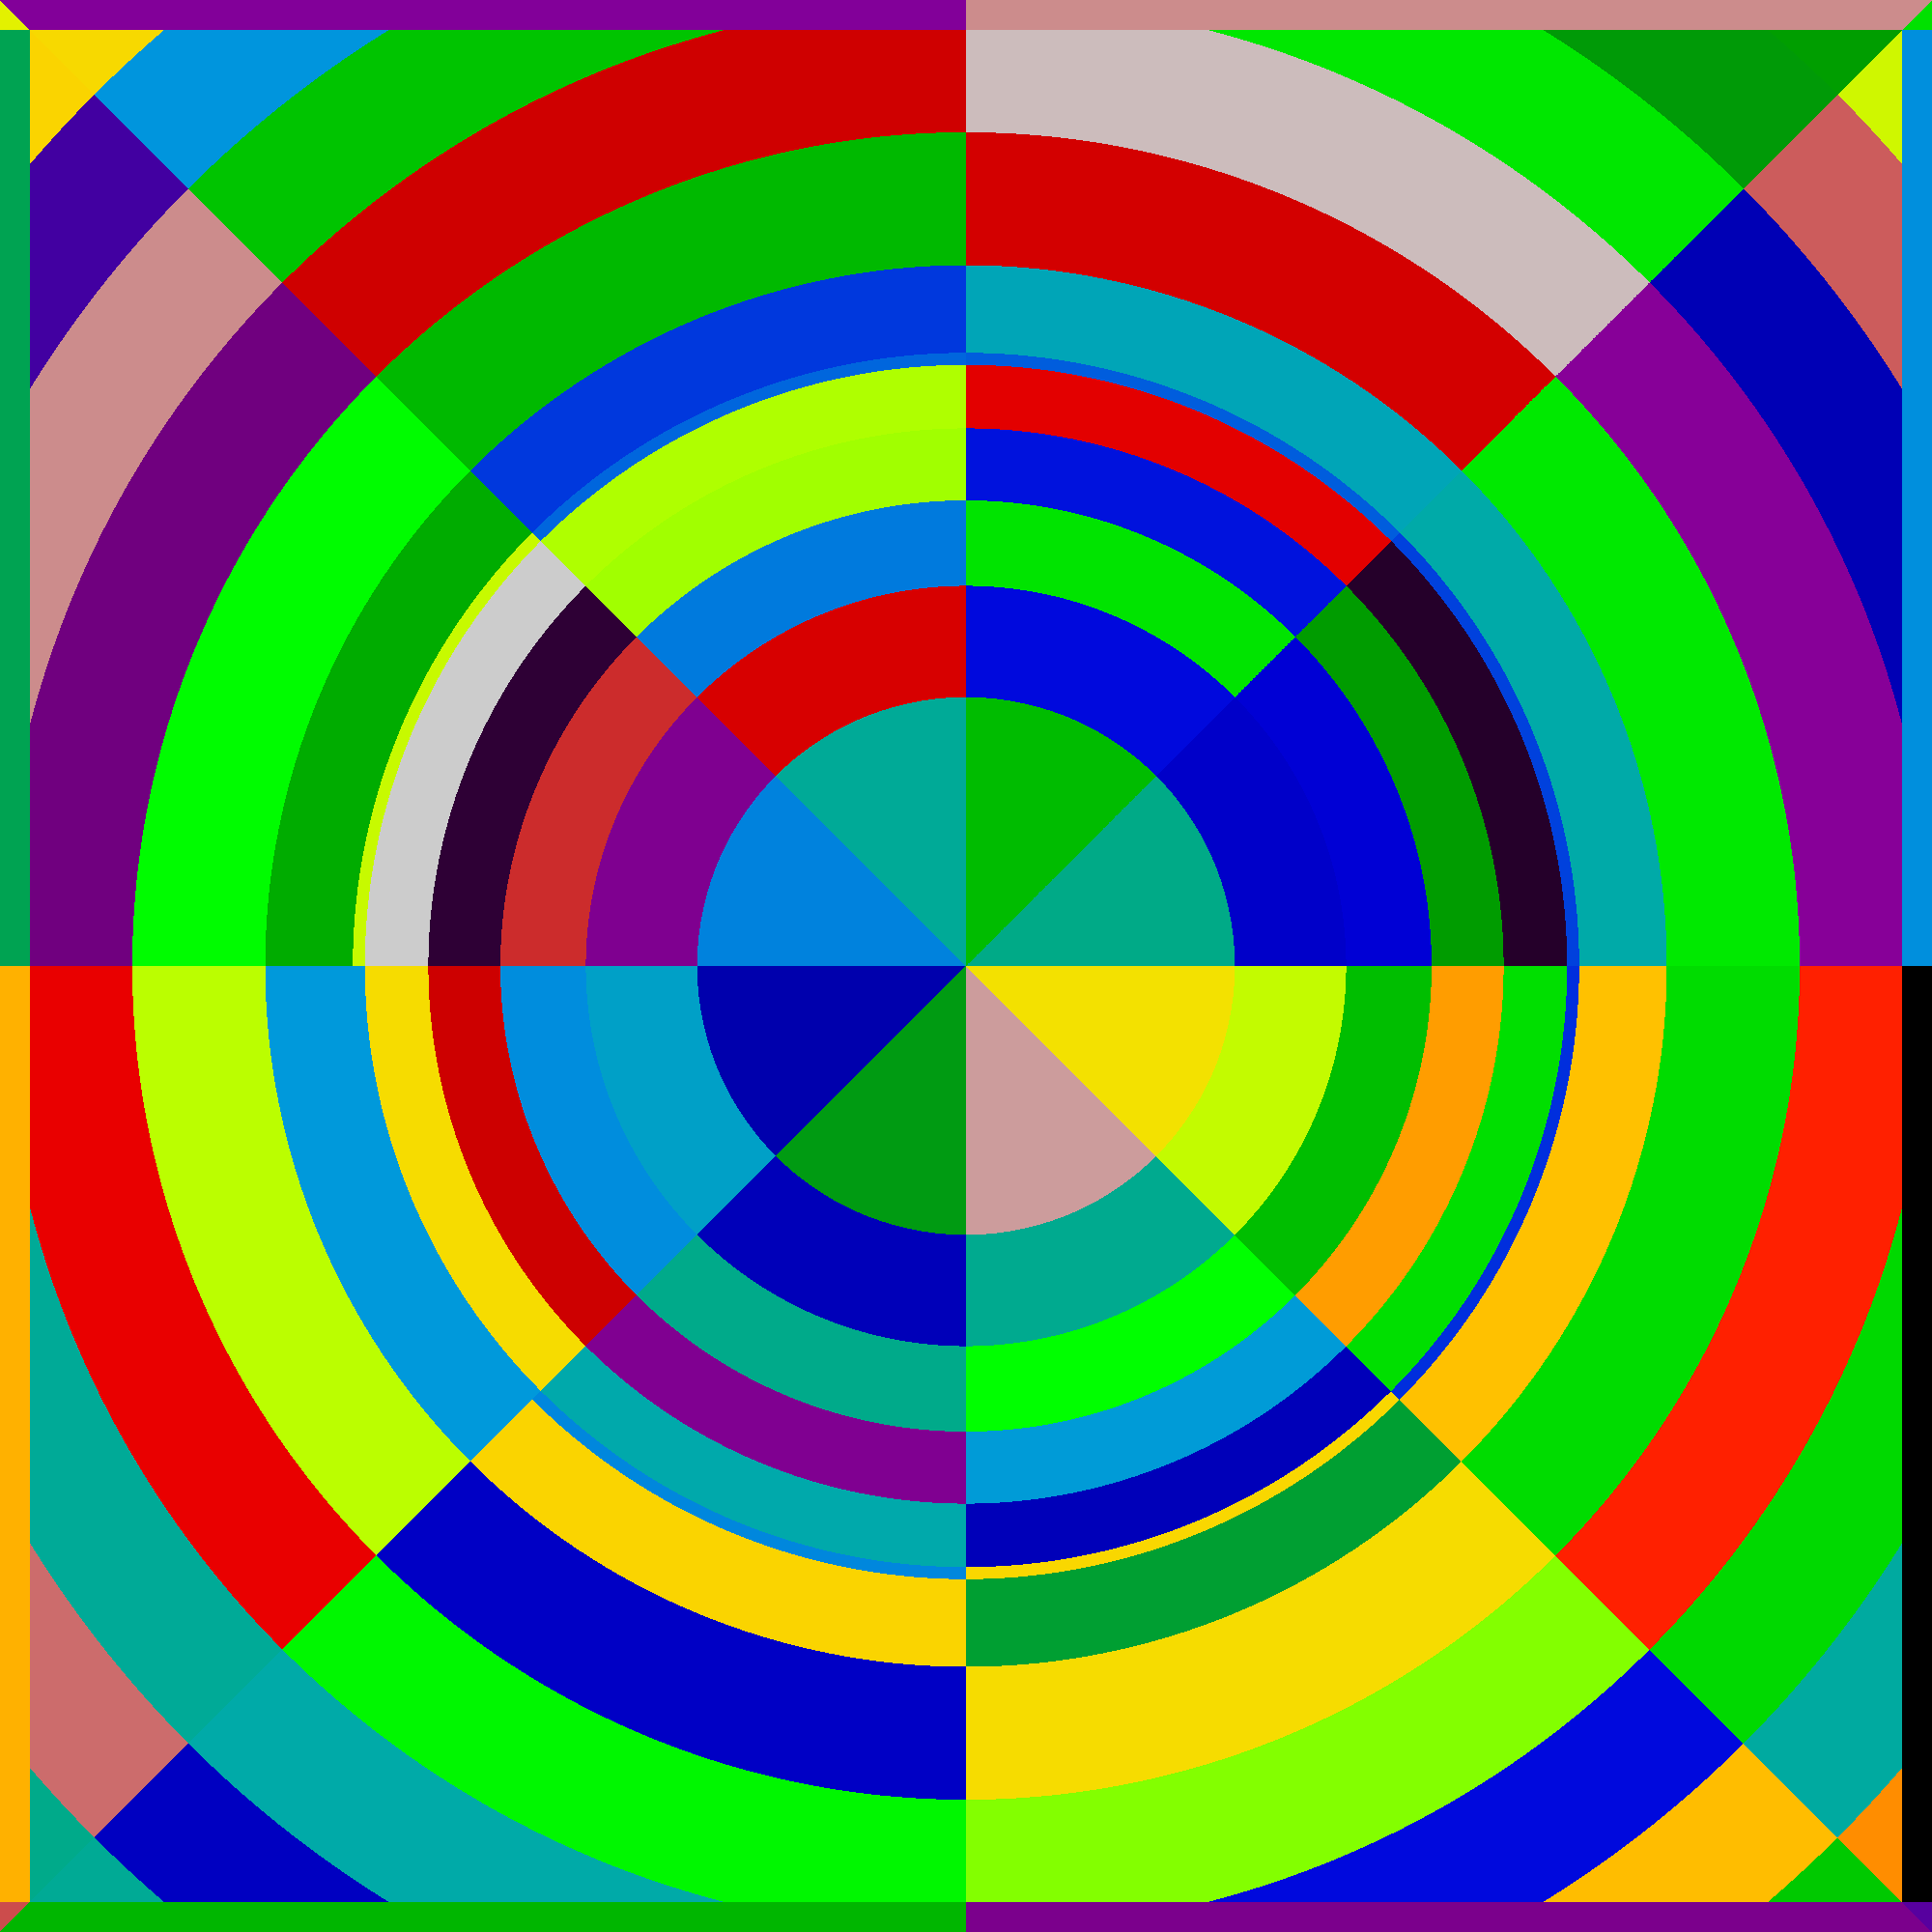
\includegraphics[width=0.9\linewidth]{figures/quantification/fsrs/fsrs-fuel-pin}
  \caption{}
  \label{fig:chap8-pin-1.6}
\end{subfigure}%
\begin{subfigure}{.5\textwidth}
  \centering
  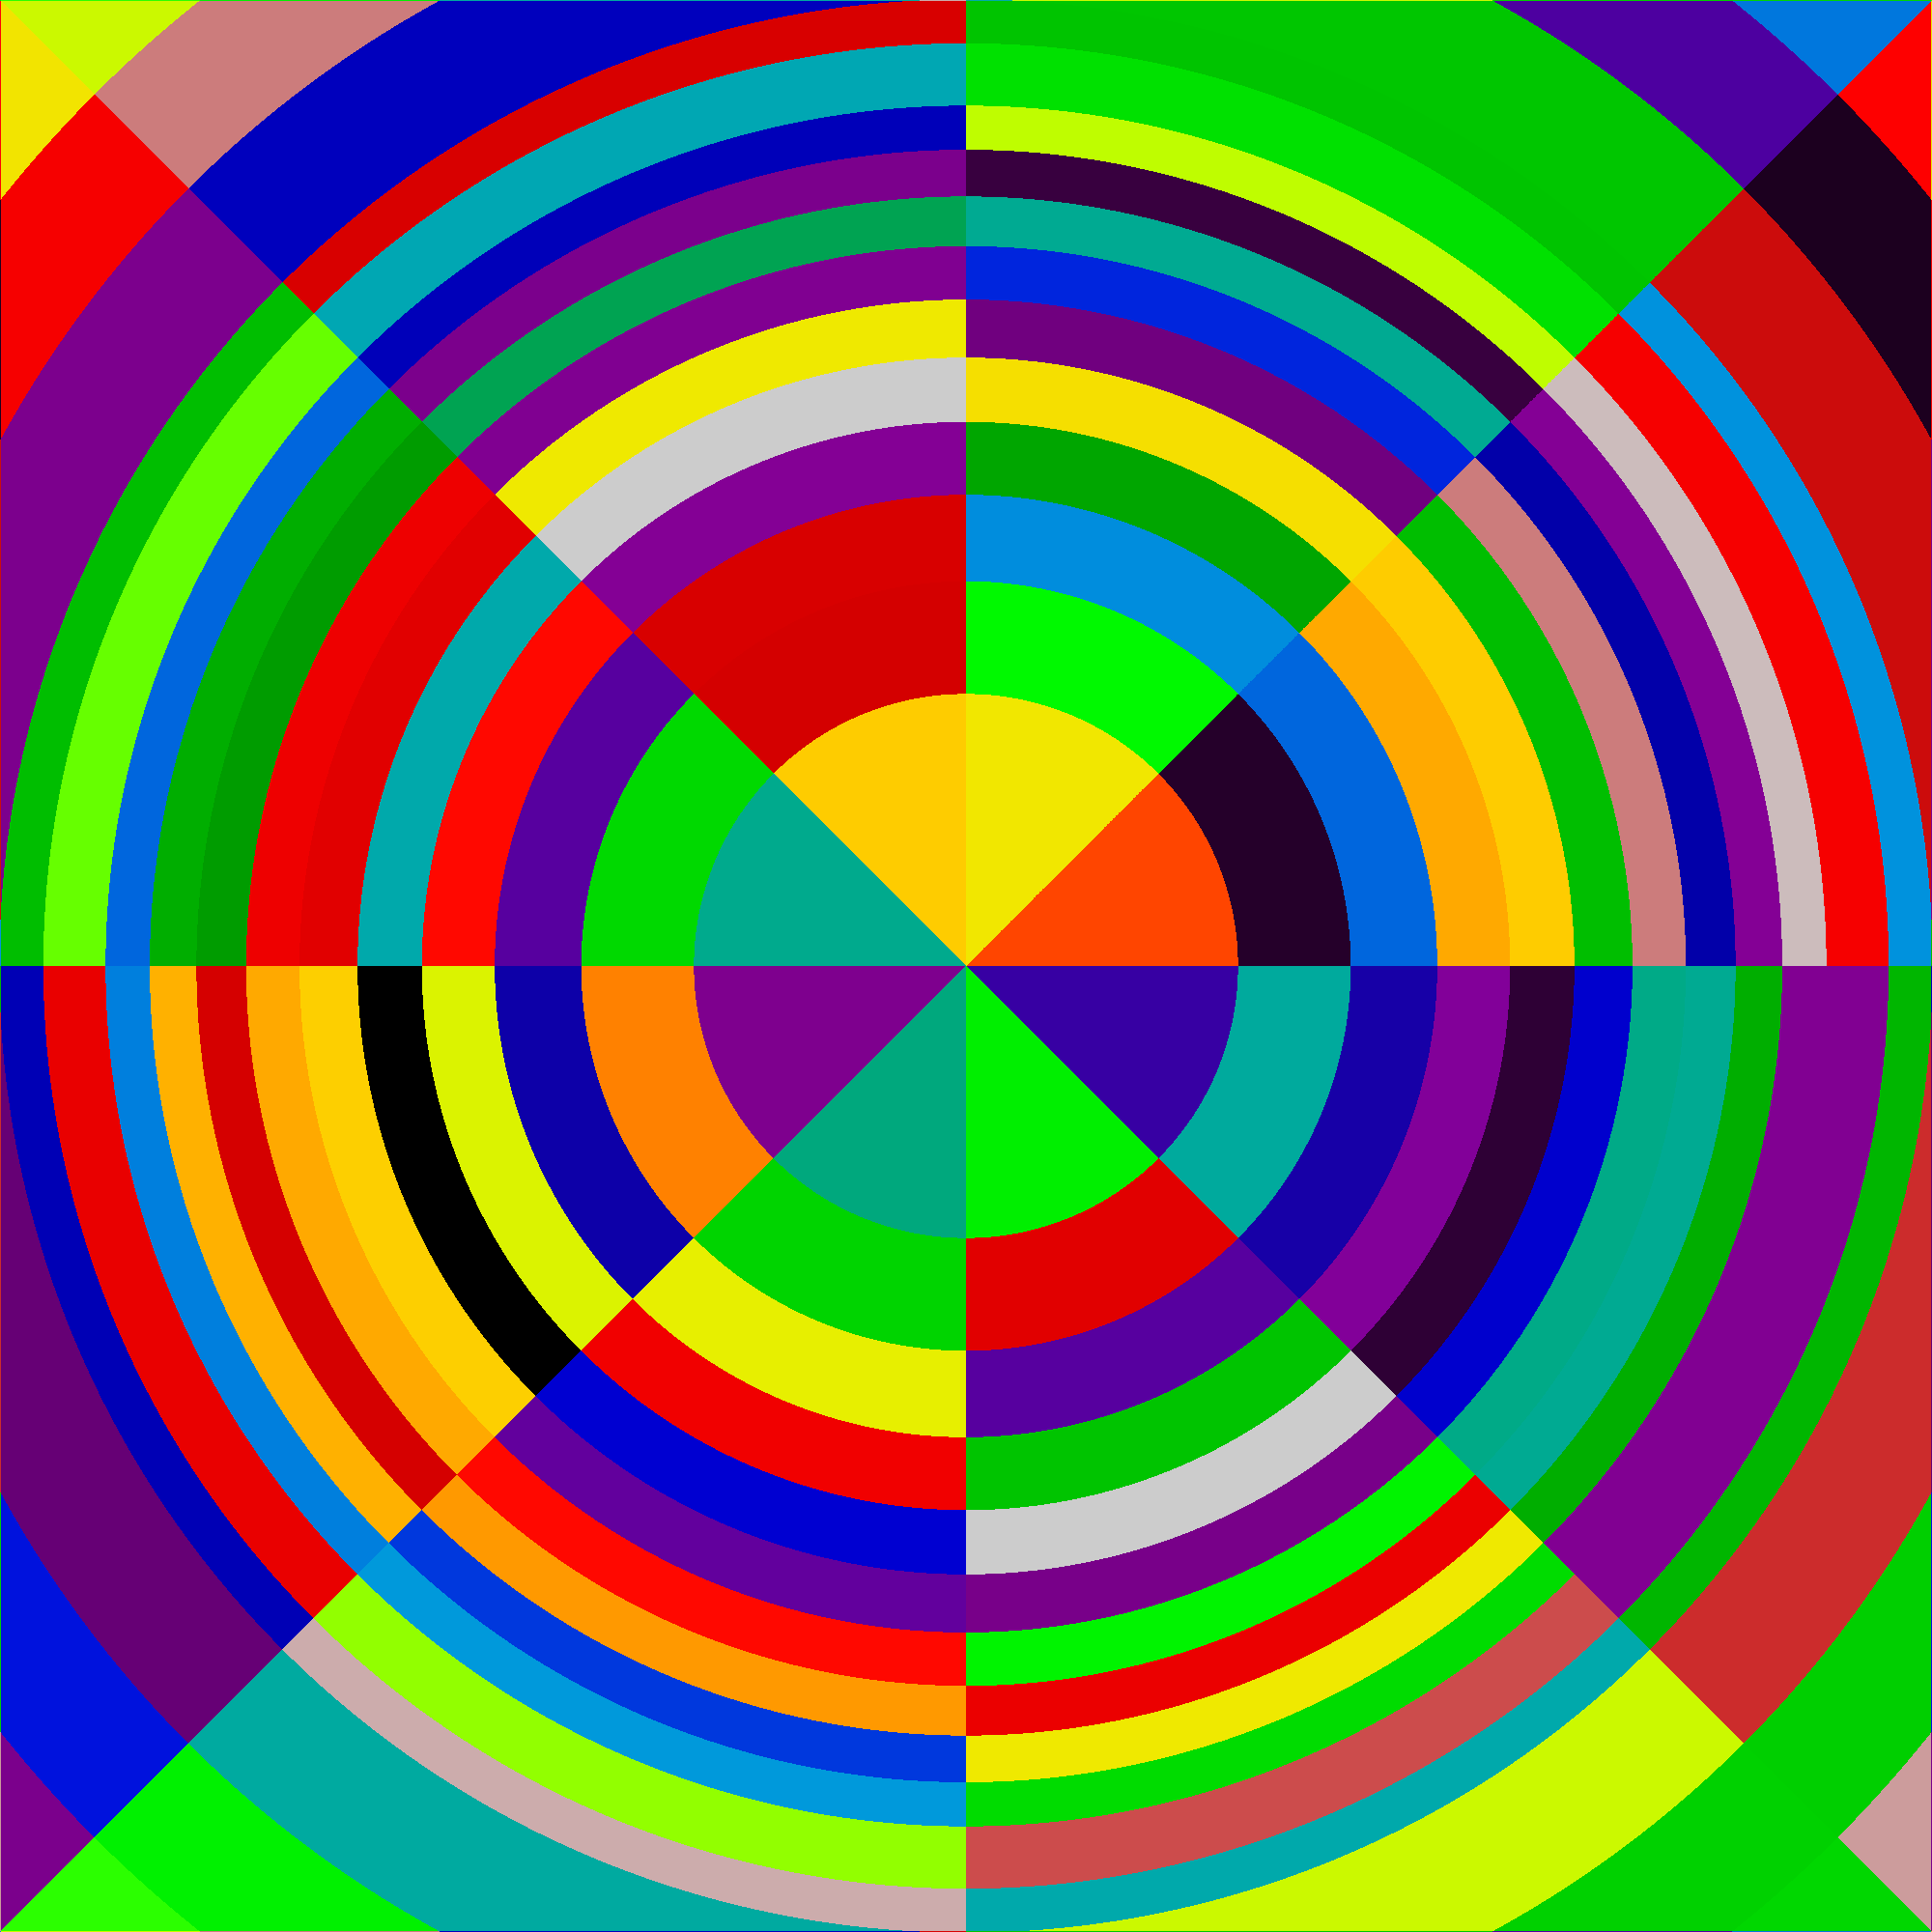
\includegraphics[width=0.9\linewidth]{figures/quantification/fsrs/fsrs-crgt}
  \caption{}
  \label{fig:chap8-pin-crgt}
\end{subfigure}
\begin{subfigure}{.5\textwidth}
  \centering
  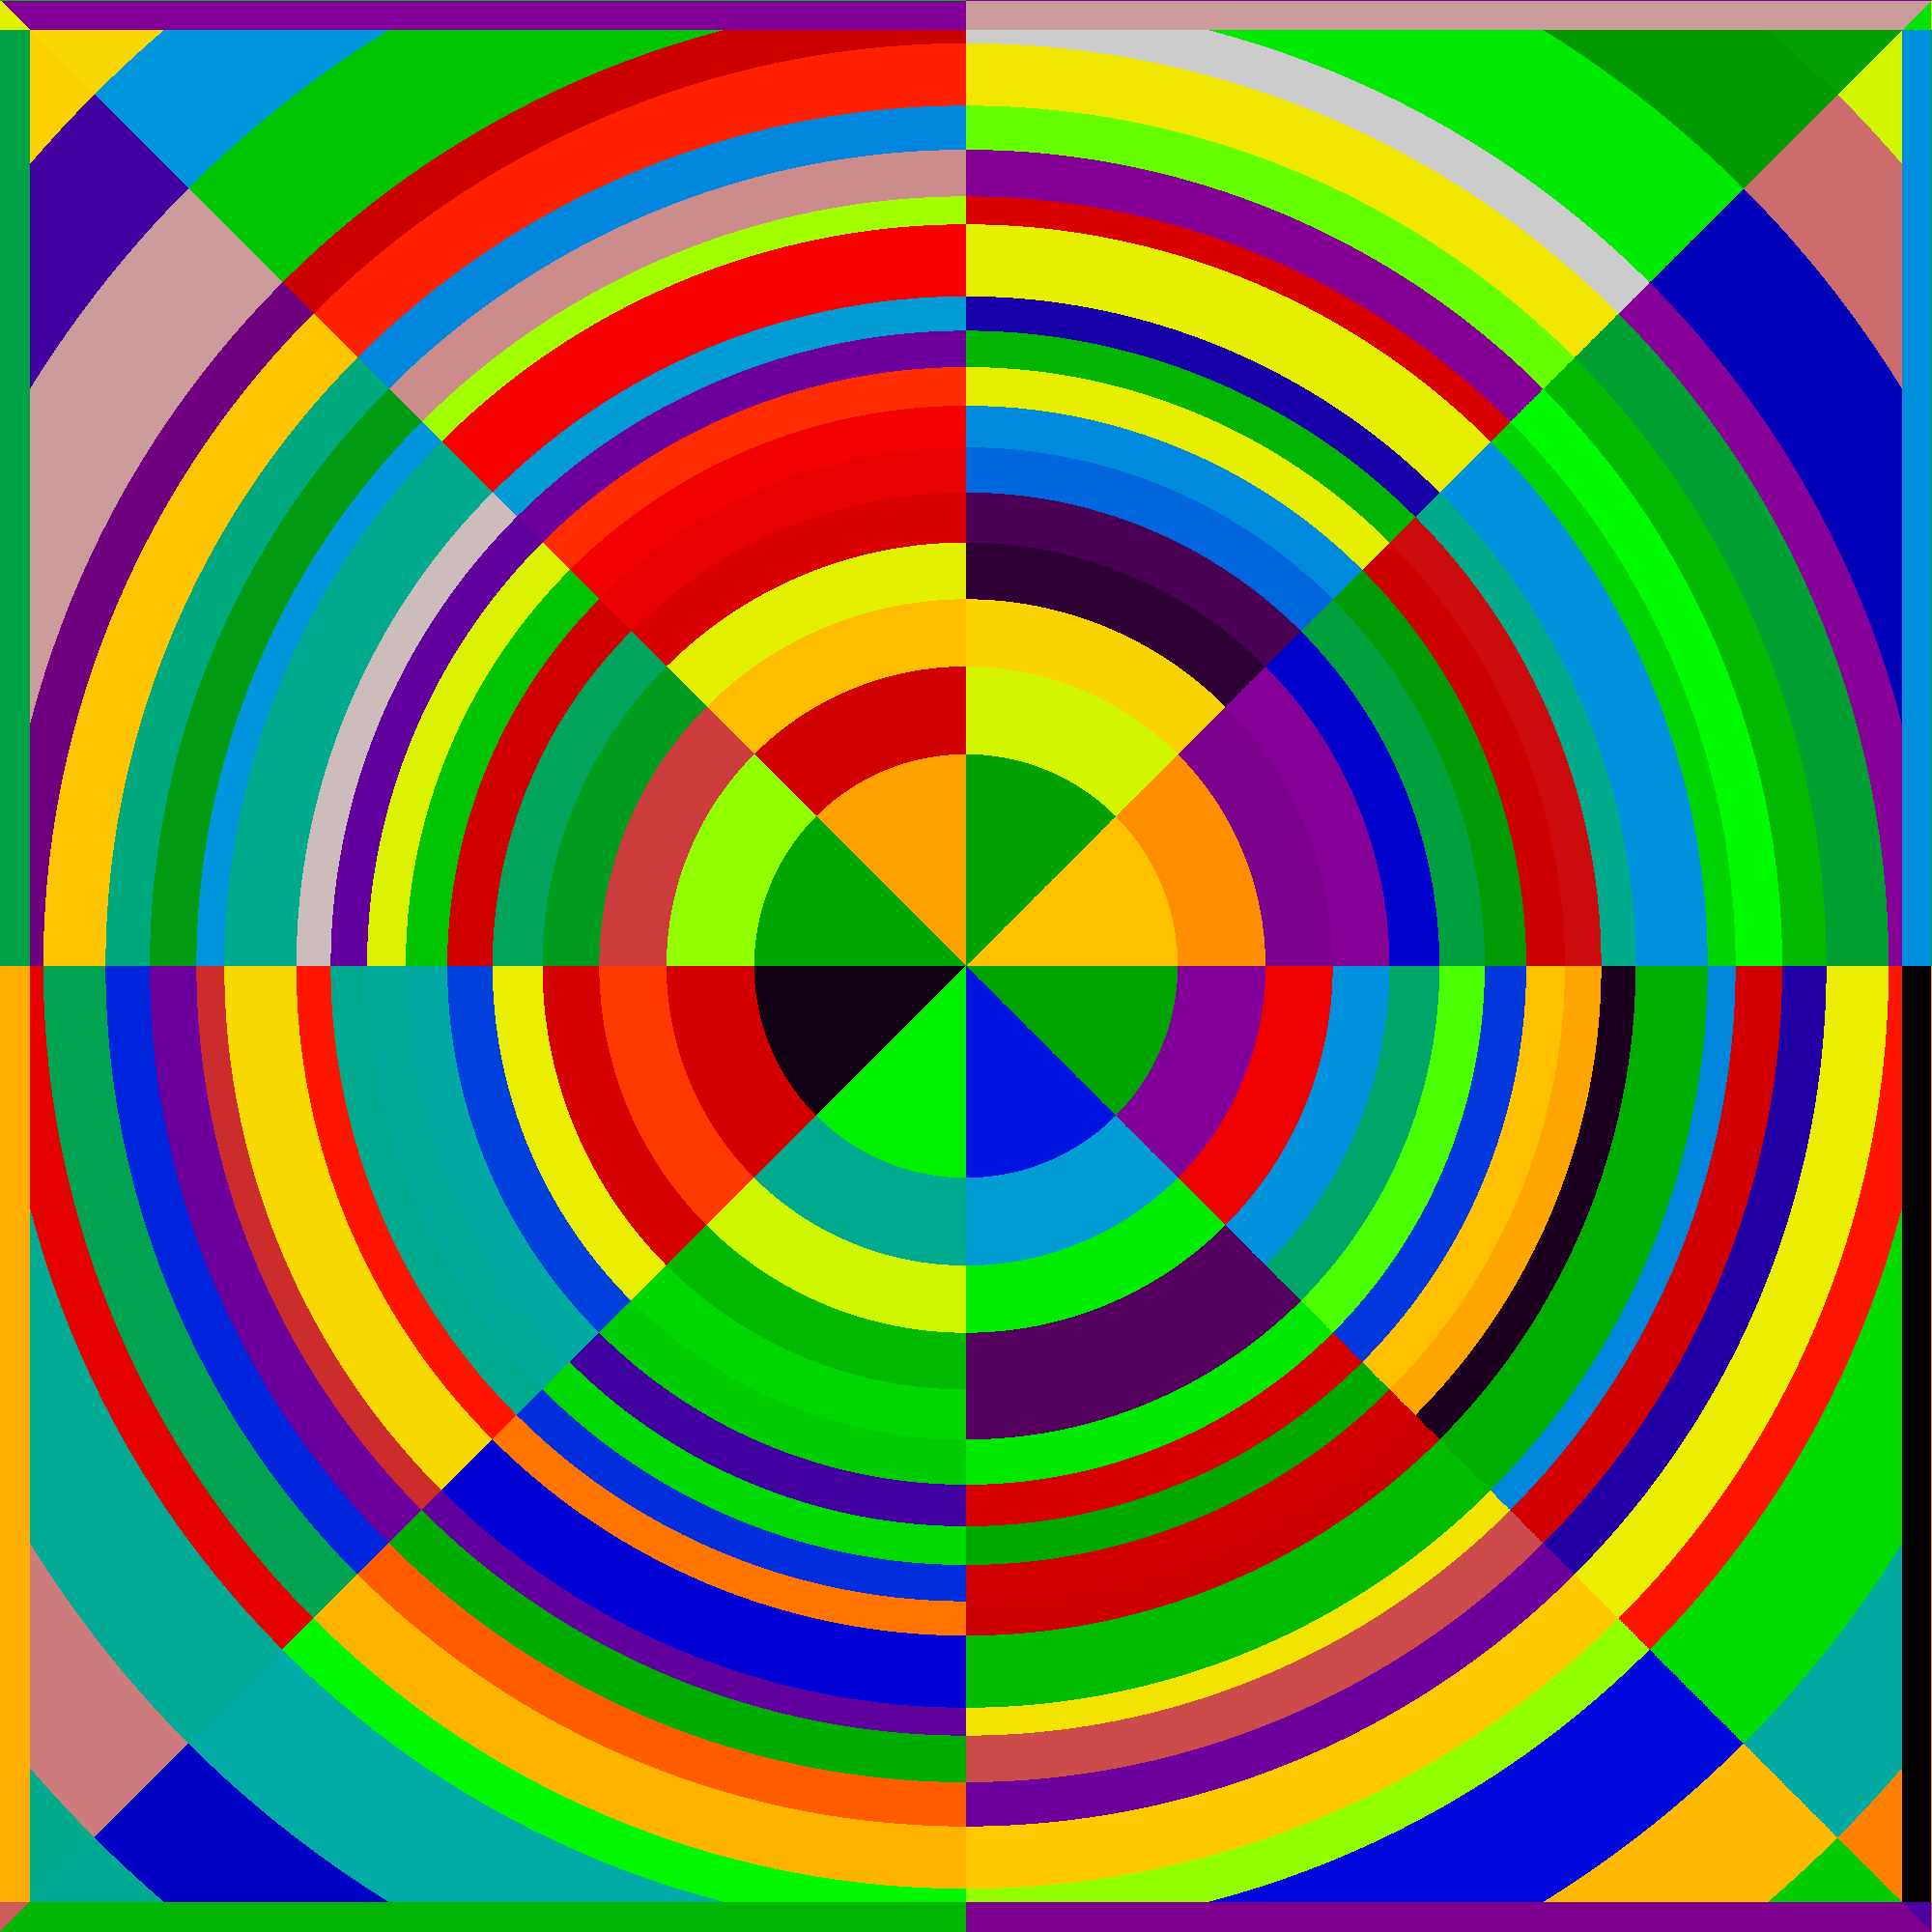
\includegraphics[width=0.9\linewidth]{figures/quantification/fsrs/fsrs-instr-tube}
  \caption{}
  \label{fig:chap8-instr-tube}
\end{subfigure}%
\begin{subfigure}{.5\textwidth}
  \centering
  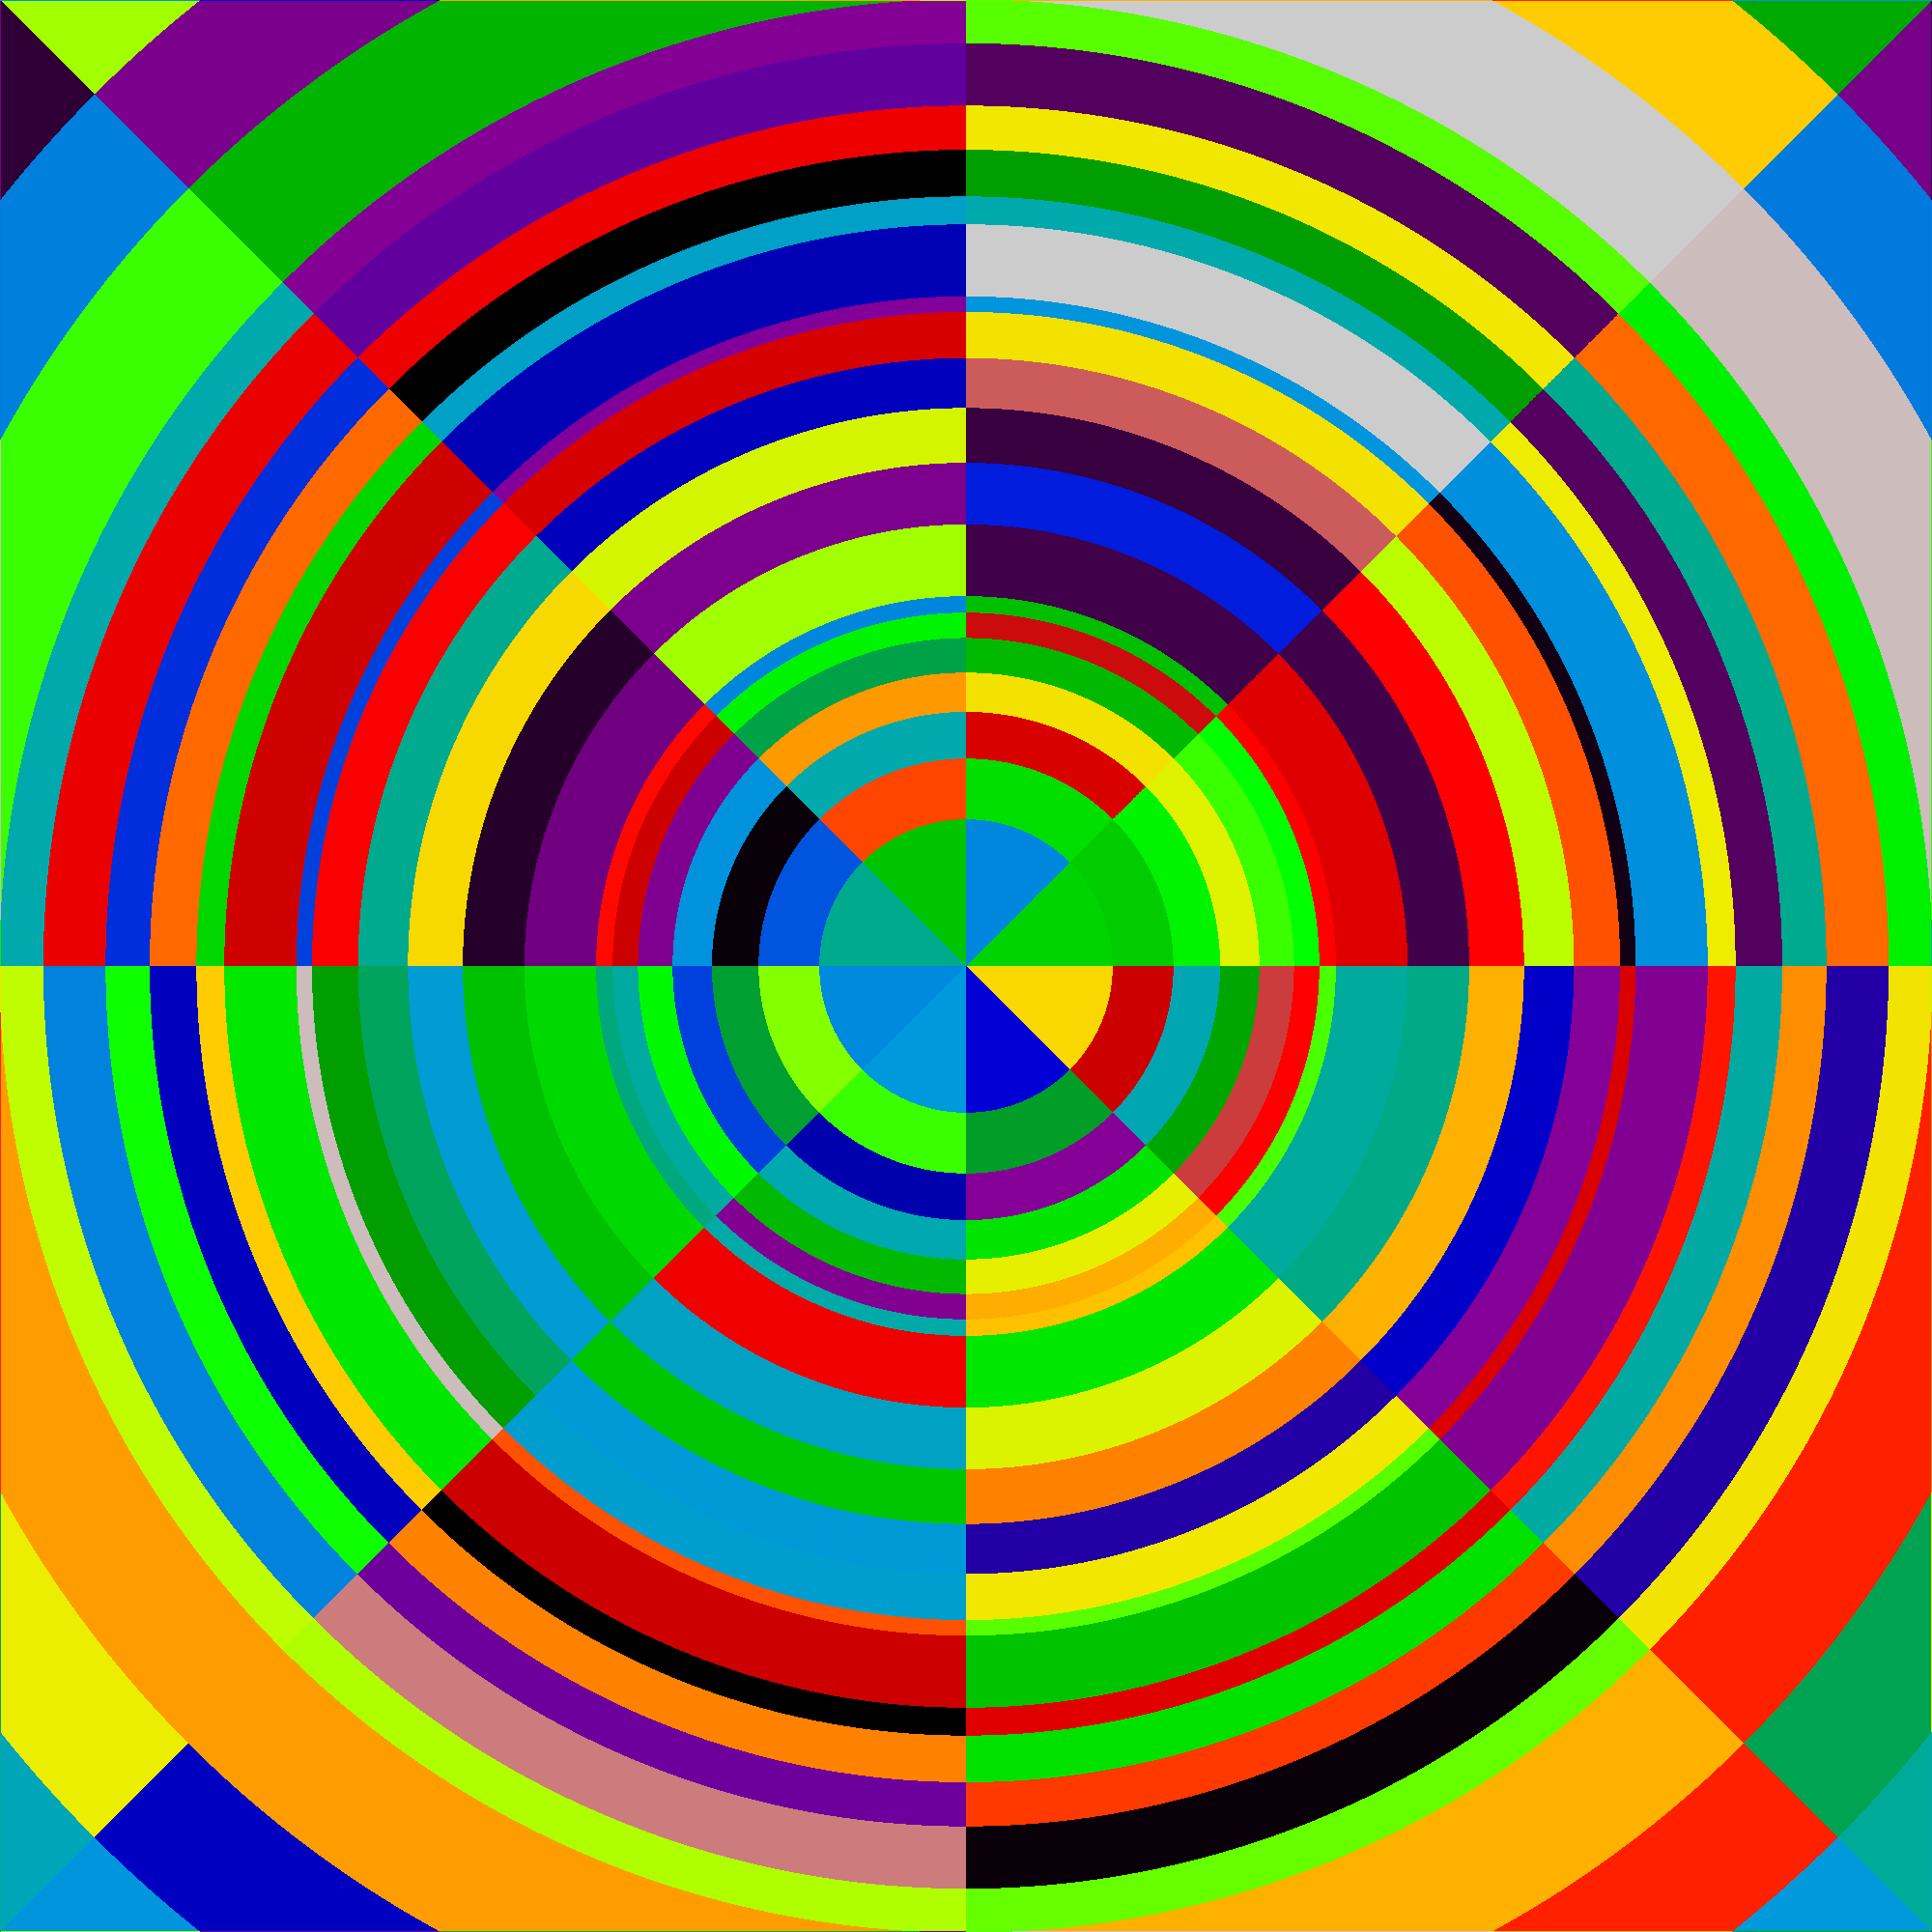
\includegraphics[width=0.9\linewidth]{figures/quantification/fsrs/fsrs-bp}
  \caption{}
  \label{fig:chap8-bp}
\end{subfigure}%
\caption[BEAVRS pin cell FSR discretization]{1.6\% enriched fuel pin (a), control rod guide tube (b), instrument tube (c) and burnable poison (d).}
\label{fig:chap8-pin-cell-fsrs}
\end{figure}

\begin{figure}[h!]
\centering
\begin{subfigure}{0.45\textwidth}
  \centering
  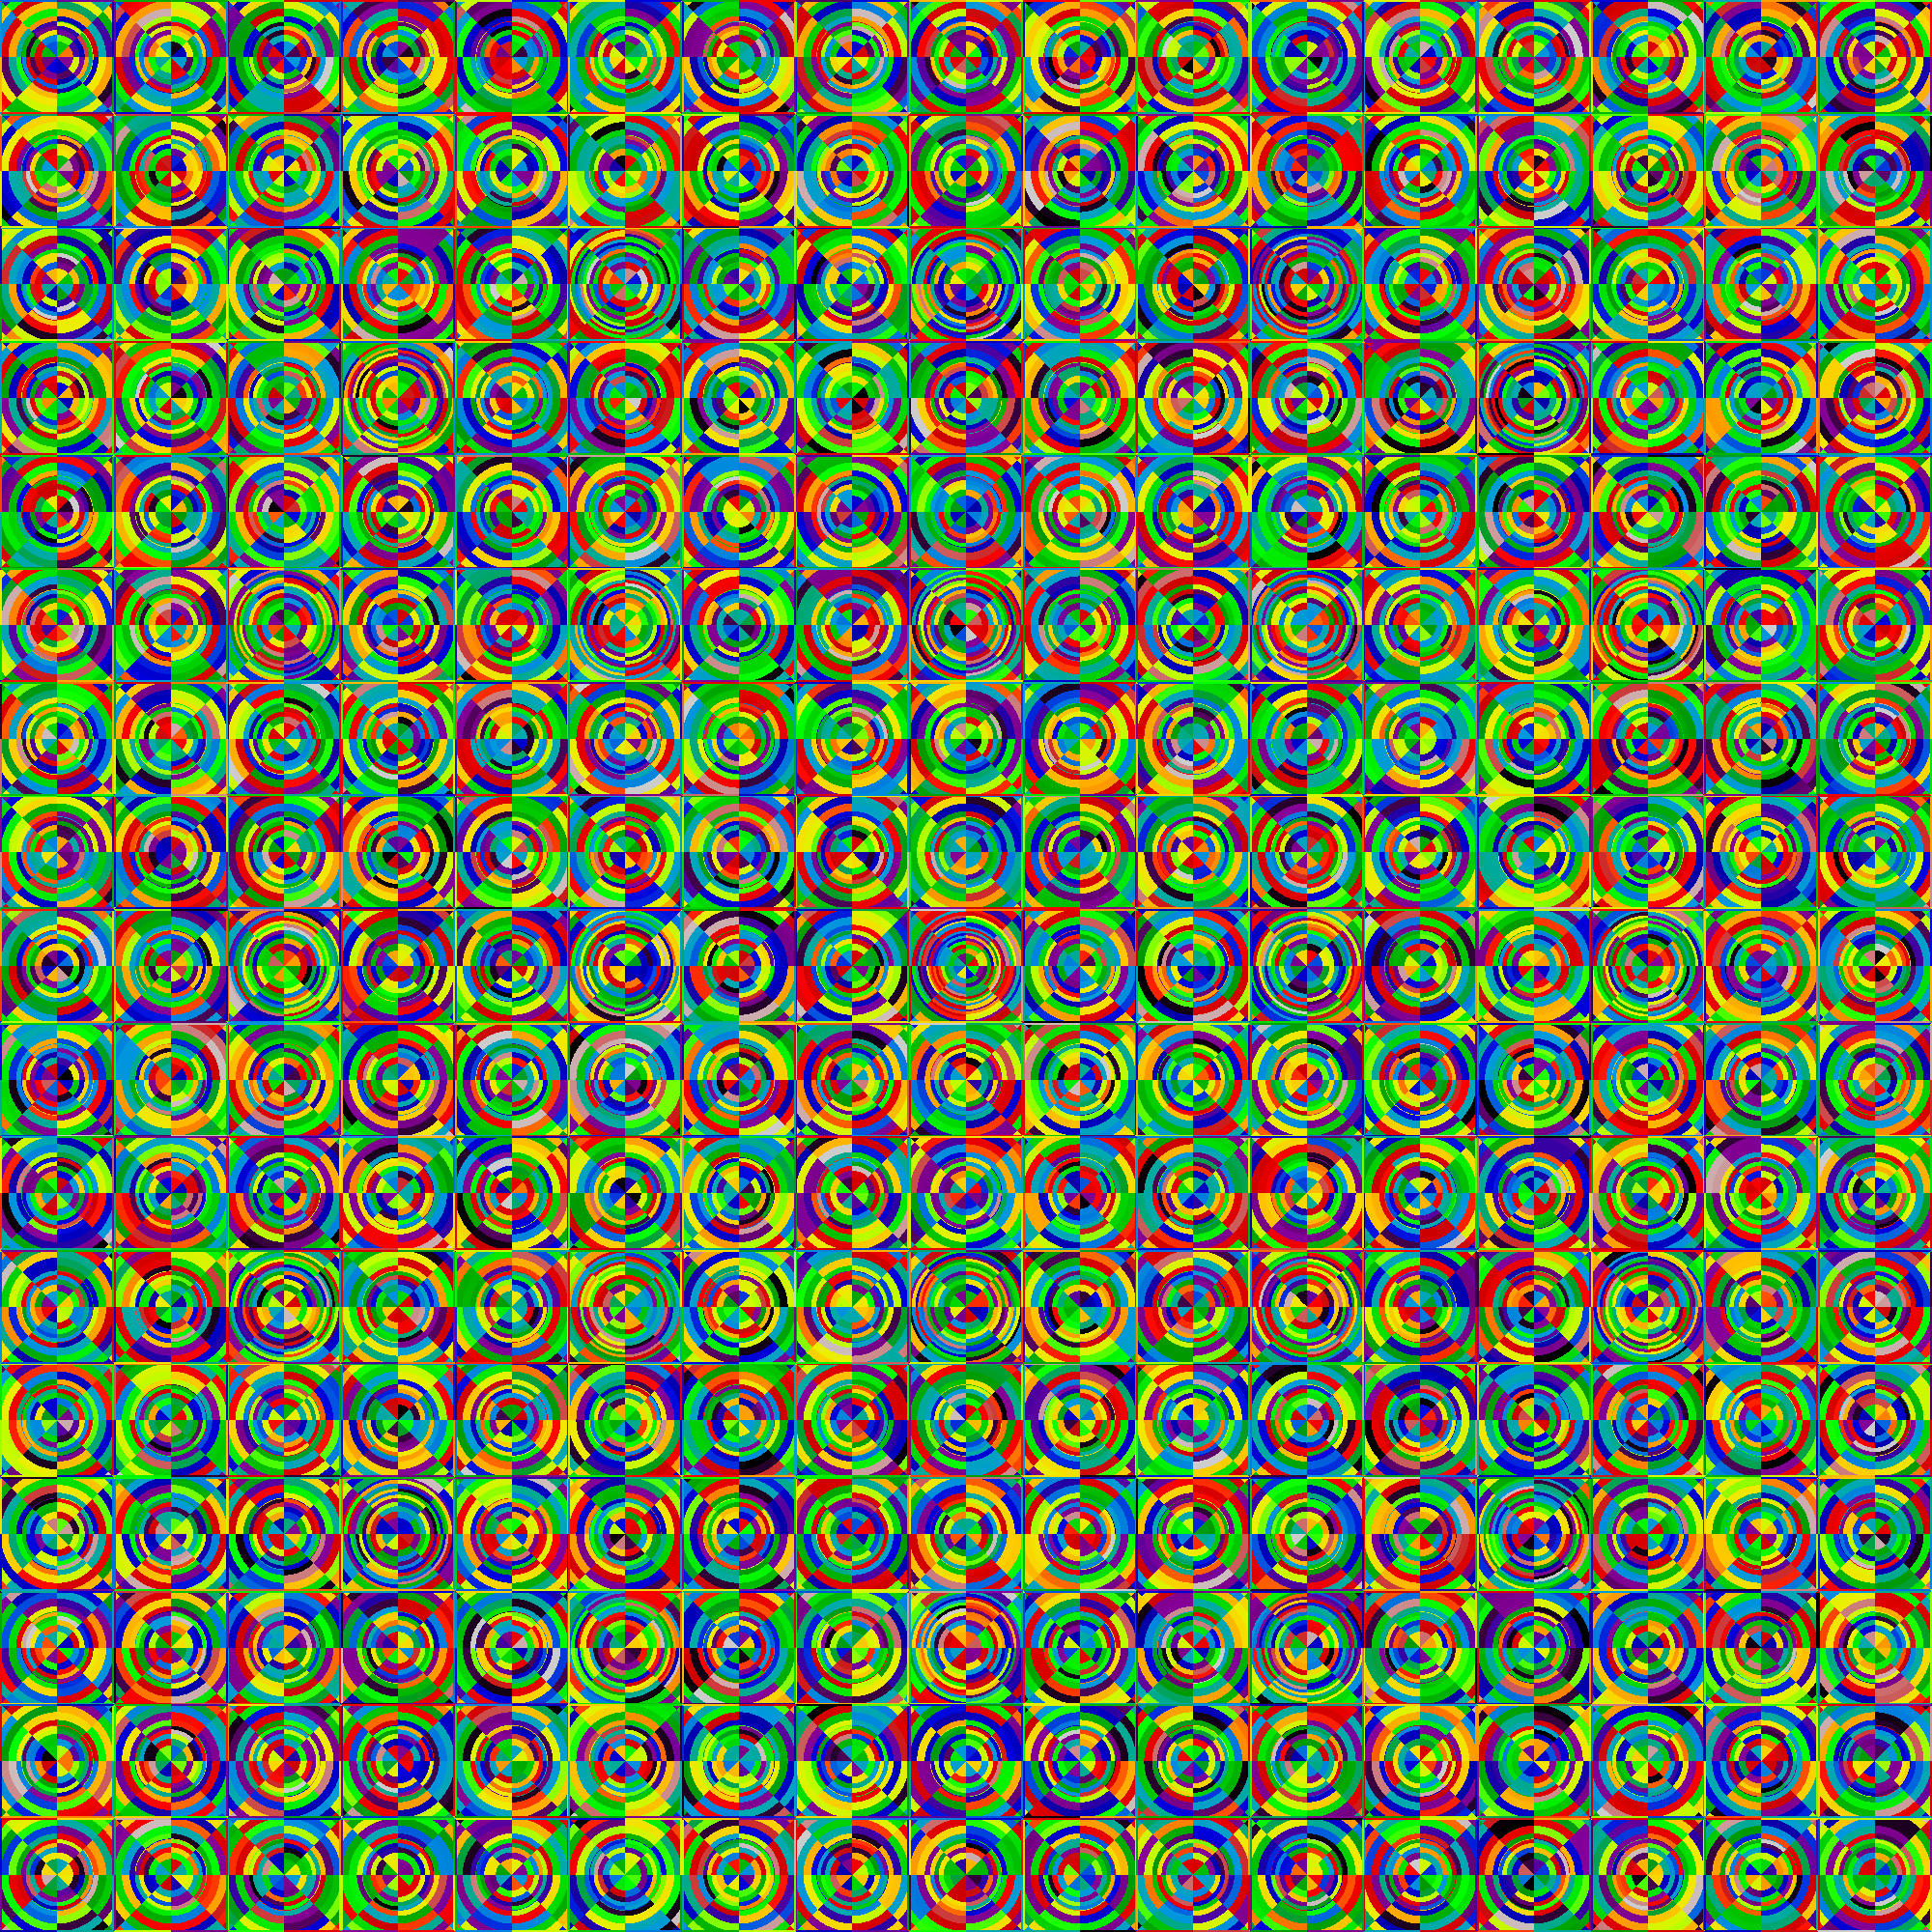
\includegraphics[width=0.8\linewidth]{figures/quantification/fsrs/fsrs-assm-16}
  \caption{}
  \label{fig:chap8-assm-1.6-fsrs}
\end{subfigure}%
\begin{subfigure}{0.45\textwidth}
  \centering
  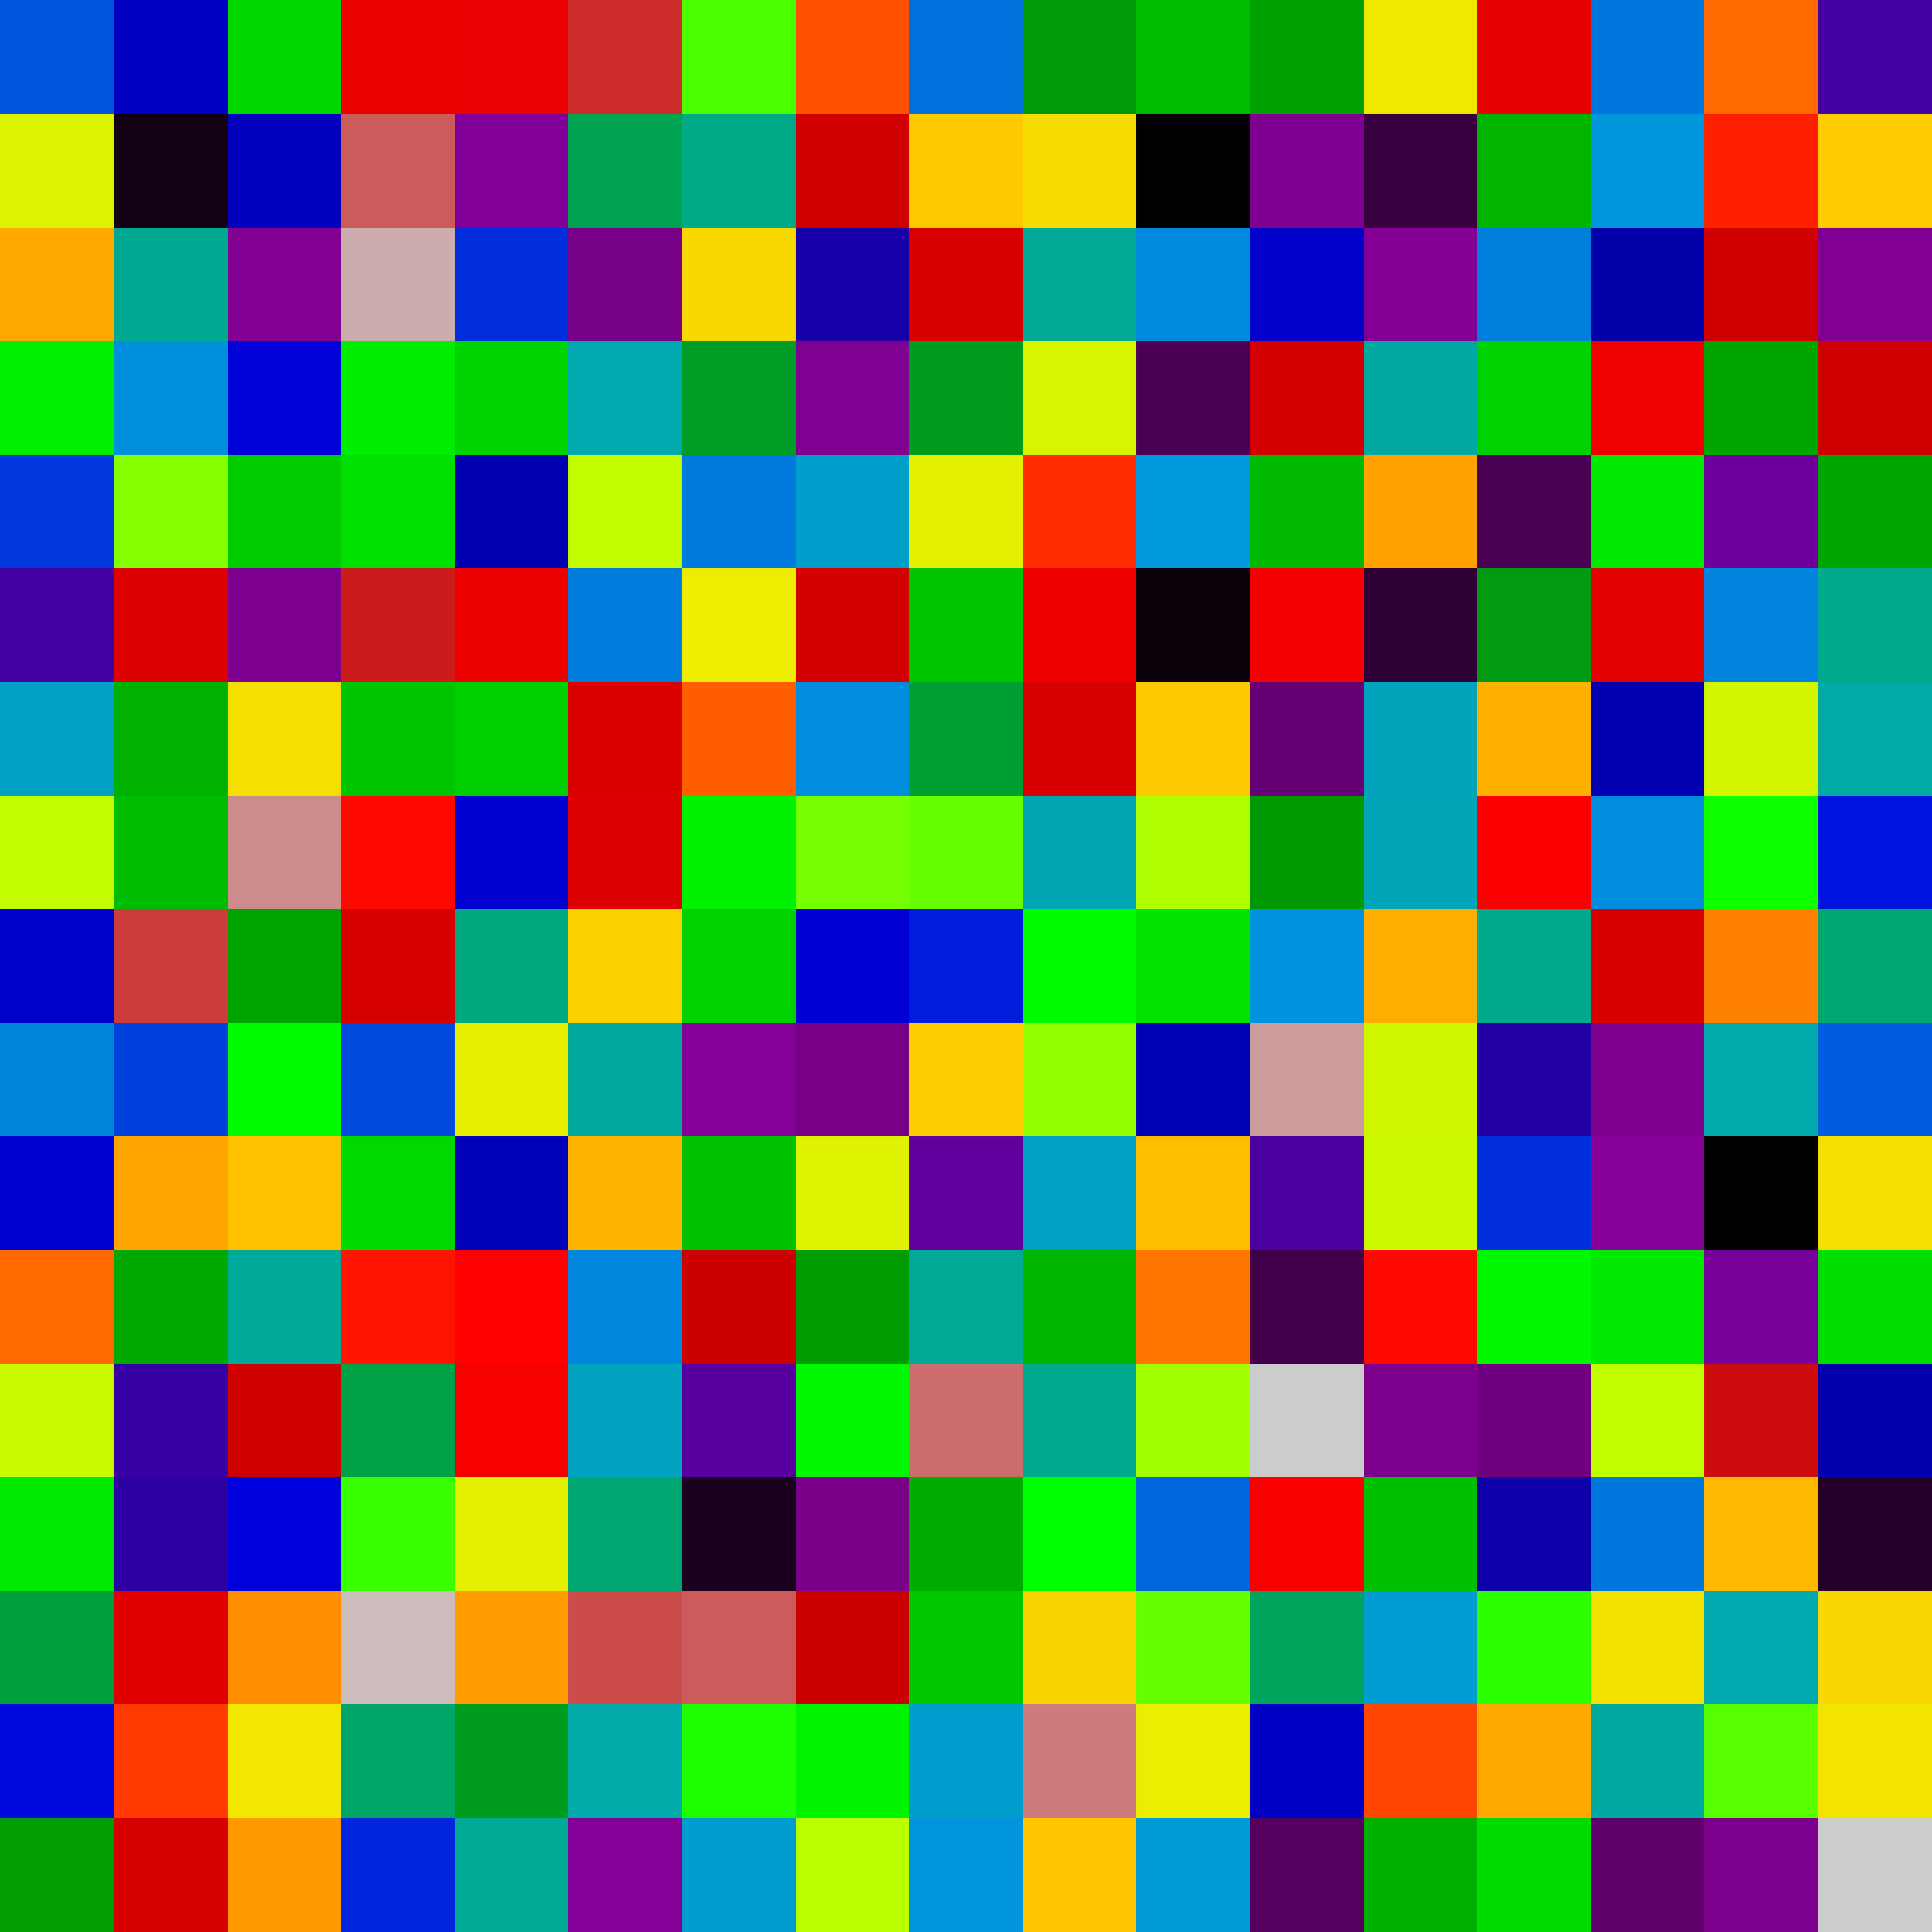
\includegraphics[width=0.8\linewidth]{figures/quantification/cmfd/cmfd-cells-assm}
  \caption{}
  \label{fig:chap8-assm-1.6-cmfd-cells}
\end{subfigure}
\begin{subfigure}{0.45\textwidth}
  \centering
  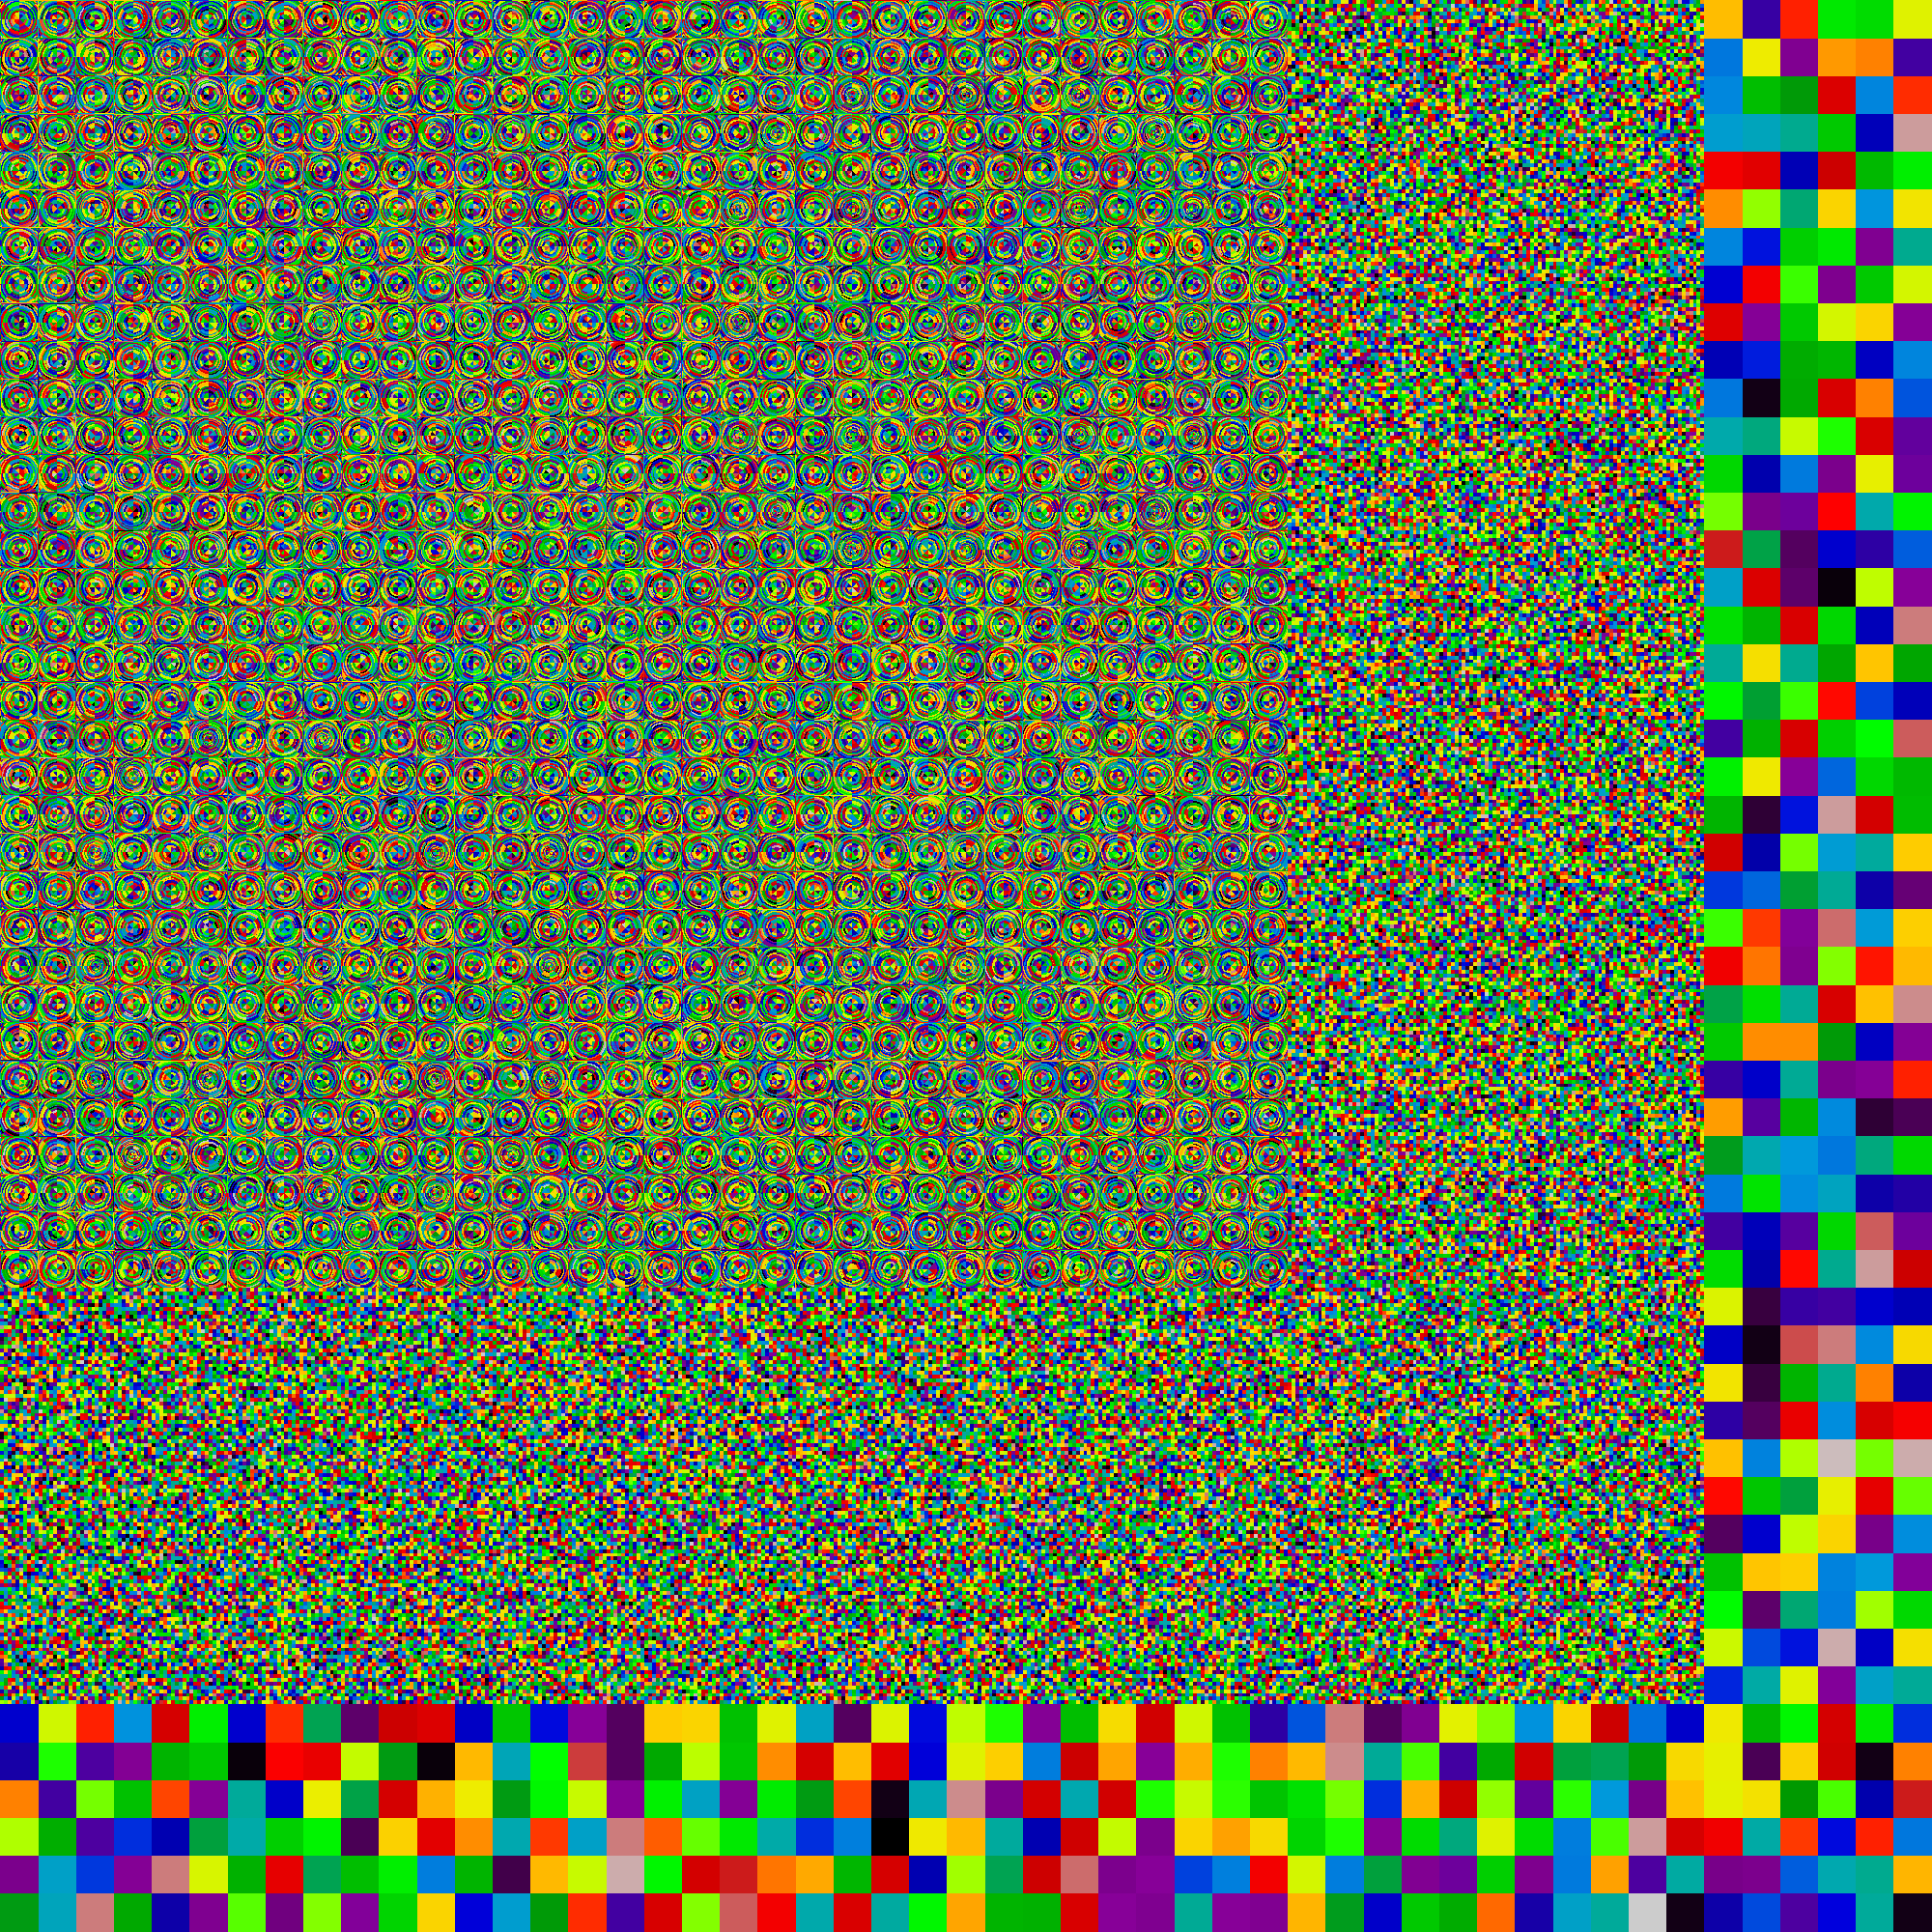
\includegraphics[width=0.8\linewidth]{figures/quantification/fsrs/fsrs-reflector}
  \caption{}
  \label{fig:chap8-reflector-fsrs}
\end{subfigure}%
\begin{subfigure}{0.45\textwidth}
  \centering
  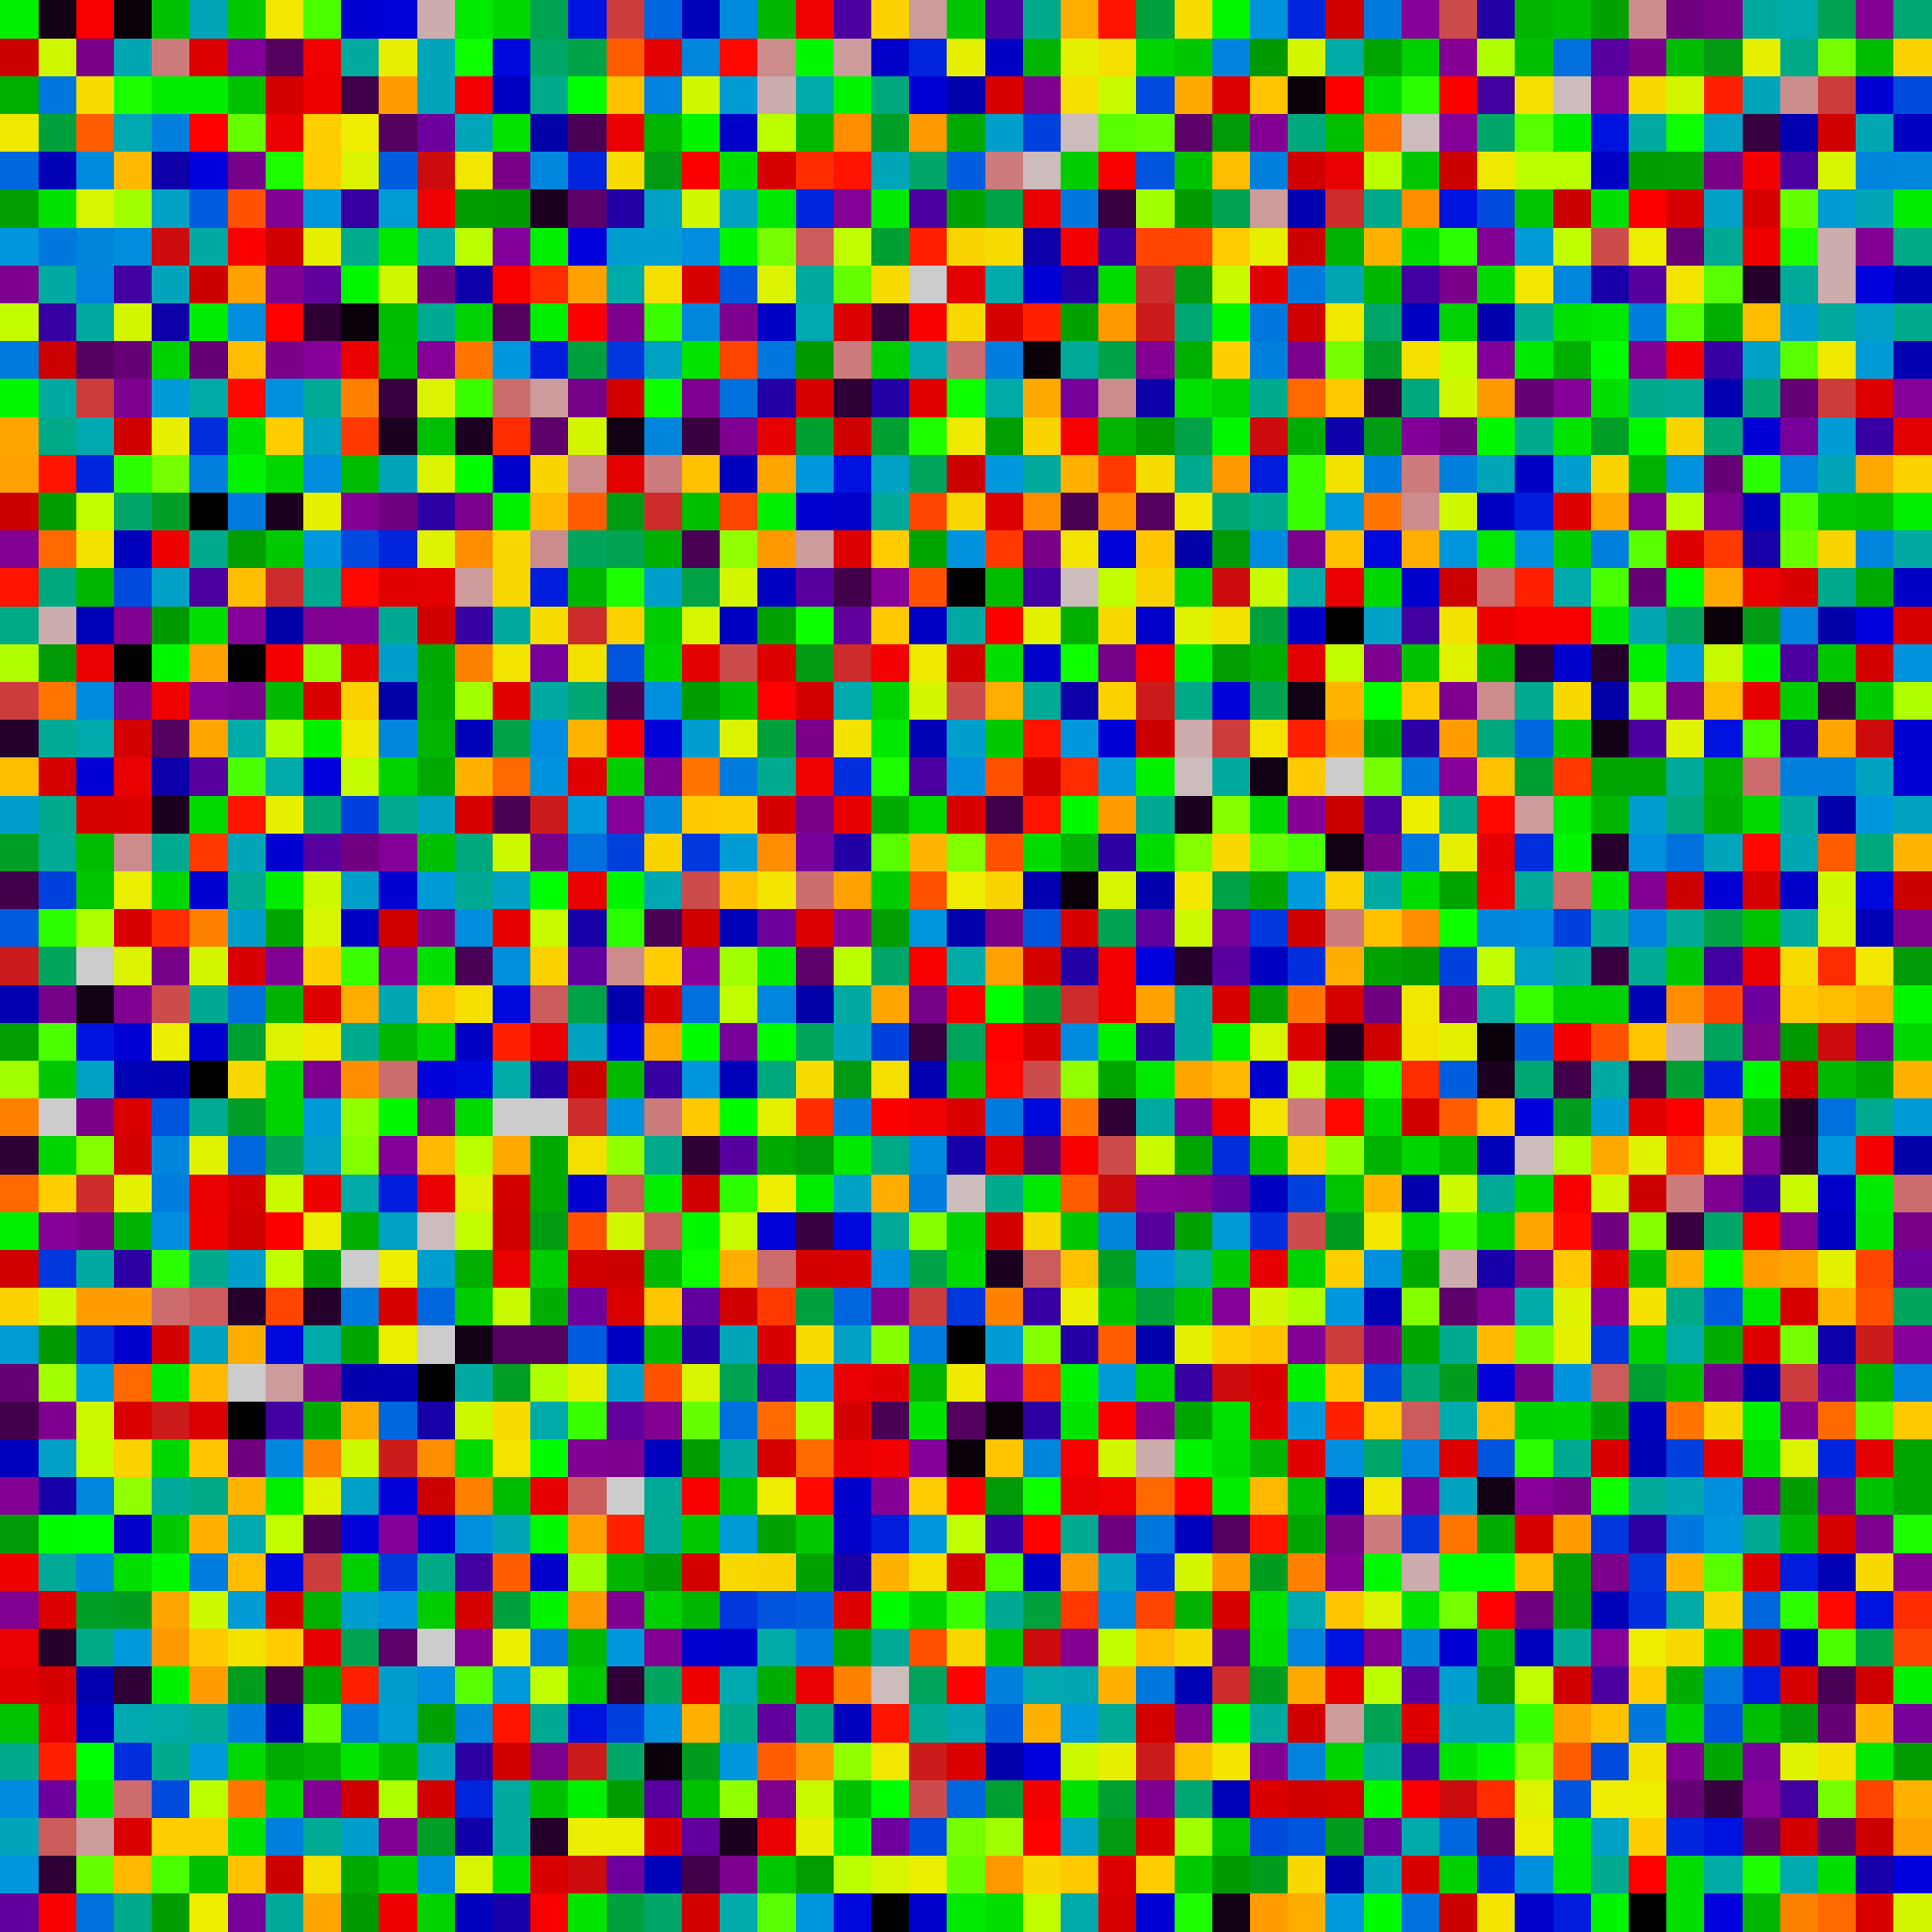
\includegraphics[width=0.8\linewidth]{figures/quantification/cmfd/cmfd-cells-reflector}
  \caption{}
  \label{fig:chap8-reflector-cmfd-cells}
\end{subfigure}
\begin{subfigure}{0.45\textwidth}
  \centering
  
\includegraphics[width=0.8\linewidth]{figures/quantification/fsrs/fsrs-full-core-quarter-pin-cmfd}
  \caption{}
  \label{fig:chap8-full-core-fsrs}
\end{subfigure}%
\begin{subfigure}{0.45\textwidth}
  \centering
  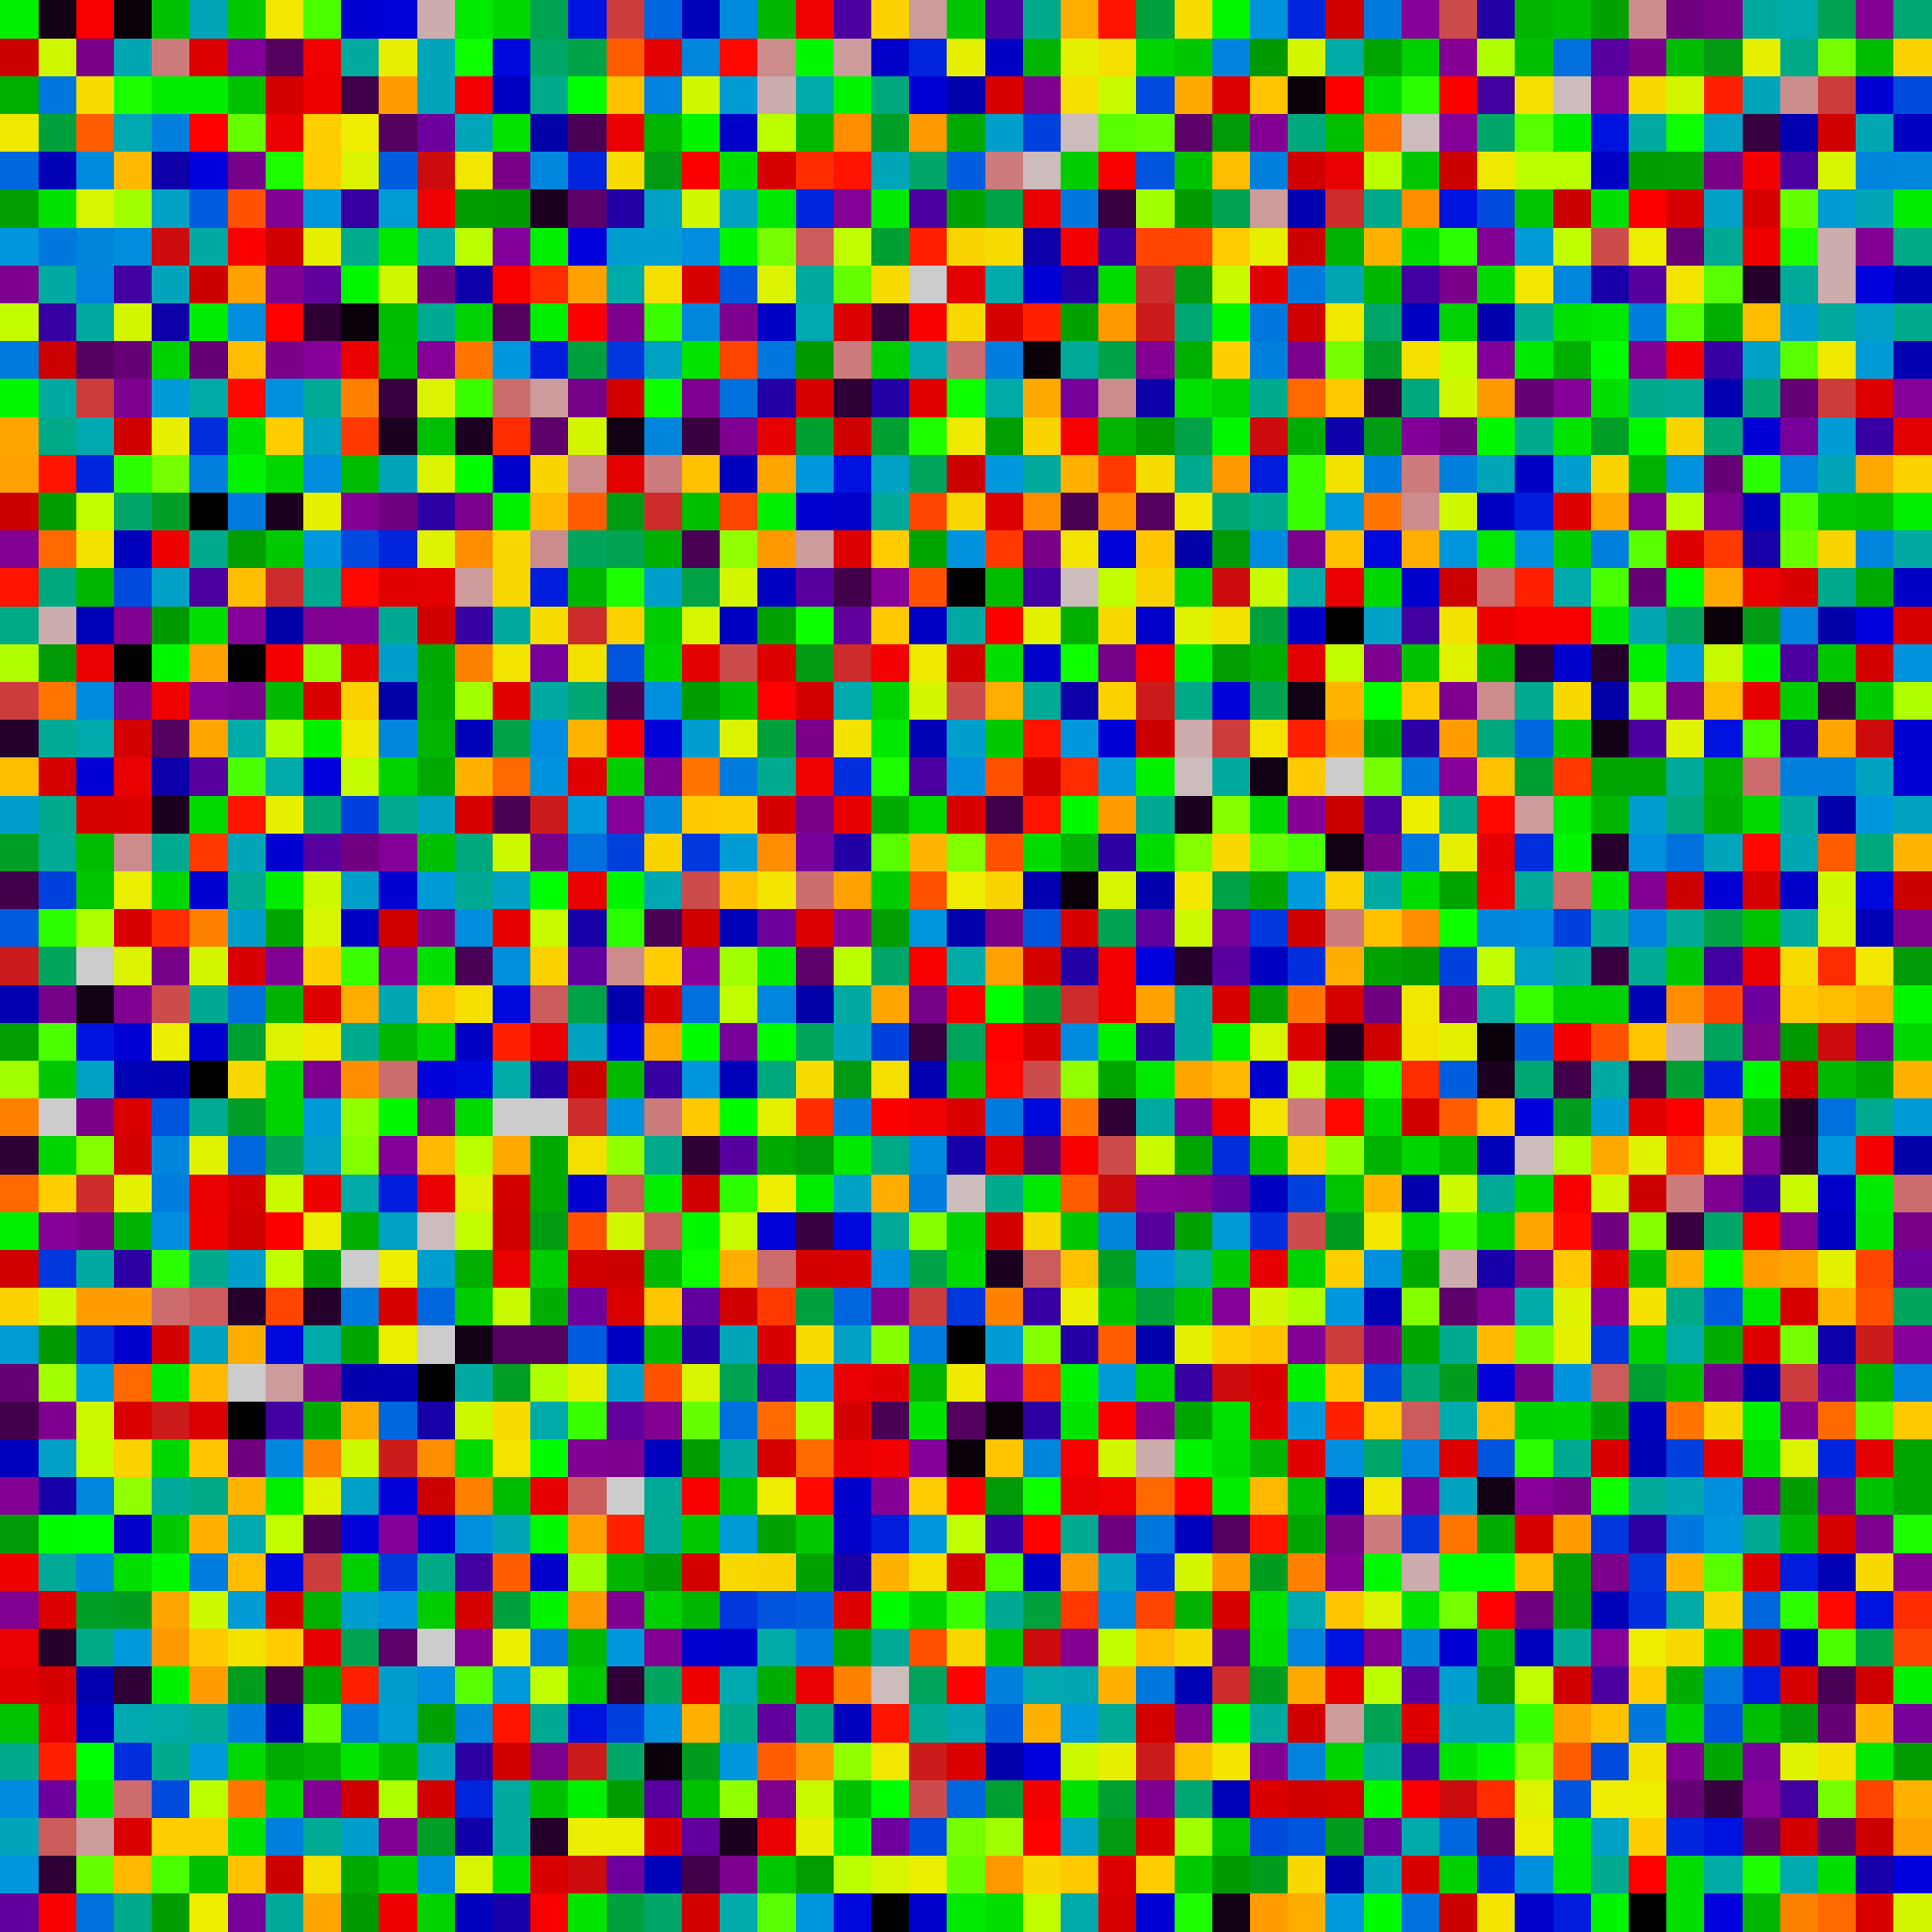
\includegraphics[width=0.8\linewidth]{figures/quantification/cmfd/cmfd-cells-full-core}
  \caption{}
  \label{fig:chap8-full-core-cmfd-cells}
\end{subfigure}
\caption[FSR discretization and CMFD cells for heterogeneous benchmarks]{\ac{FSR} discretization and \ac{CMFD} cells for a fuel assembly (a) and (b), a 2$\times$2 colorset with reflector (c) and (d), and the 2D quarter core \ac{BEAVRS} benchmark (e) and (f), respectively.}
\label{fig:chap8-assm-fsrs-cmfd-cells}
\end{figure}

%%%%%%%%%%%%%%%%%%%%%%%%%%%%%%%%%%%%
\subsection{\ac{CMFD}}
\label{subsec:chap8-cmfd}

first paragraph:
-coarse pin-wise spatial mesh
-same energy group structure as in \ac{MOC}
-$k$-Nearest updated with 3 neighbors


%%%%%%%%%%%%%%%%%%%%%%%%%%%%%%%%%%%%%%%%%%%%%%%%%%%%%%%%%%%%%%%%%%%%%%%%%%%%%%%
\section{Analysis of Multi-Group Results}
\label{sec:chap8-mg-results}


%%%%%%%%%%%%%%%%%%%%%%%%
\subsection{Eigenvalues}
\label{subsec:chap8-eigenvalues}

\begin{table}[h!]
  \centering
  \caption[OpenMOC eigenvalue bias for heterogeneous benchmarks]{OpenMOC eigenvalue bias $\Delta\rho$ for heterogeneous benchmarks with varying spatial homogenization schemes and energy group structures.}
  \small
  \label{table:chap8-openmoc-eigenvalues}
  \vspace{6pt}
  \begin{tabular}{l l S[table-format=6.0] S[table-format=6.0] S[table-format=6.0]}
  \toprule
  \rowcolor{lightgray}
  & & \multicolumn{3}{S[table-format=6.1]}{\cellcolor{lightgray} {$\bm{\Delta\rho}$ \textbf{[pcm]}}} \\
  \multirow{-2}{*}{\cellcolor{lightgray} \bf Benchmark} &
  \multirow{-2}{*}{\cellcolor{lightgray} \bf \ac{MGXS} Scheme} &
  \multicolumn{1}{c}{{\cellcolor{lightgray} \bf 2-Group}} &
  \multicolumn{1}{c}{{\cellcolor{lightgray} \bf 8-Group}} &
  \multicolumn{1}{c}{{\cellcolor{lightgray} \bf 70-Group}} \\
  \midrule
\multirow{3}{*}{\parbox{2.5cm}{1.6\% Assm}} & Infinite & 217 & 3 & -163 \\
& Null & 83 & -50 & -136 \\
& Degenerate & 88 & -50 & -136 \\
  \midrule
\multirow{3}{*}{\parbox{2.5cm}{3.1\% Assm}} & Infinite & 180 & -34 & -195 \\
& Null & 93 & -54 & -159 \\
& Degenerate & 99 & -54 & -159 \\
  \midrule
\multirow{3}{*}{\parbox{2.5cm}{3.1\% Assm w/ 20 BPs}} & Infinite & 1056 & 151 & -270 \\
& Null & -143 & -157 & -227 \\
& Degenerate & -190 & -159 & -223 \\
  \midrule
\multirow{3}{*}{\parbox{2.5cm}{2$\times$2 Colorset}} & Infinite & 1022 & -22 & -229 \\
& Null & 16 & -79 & -183 \\
& Degenerate & -11 & -80 & -181 \\
  \midrule
\multirow{3}{*}{\parbox{2.5cm}{2$\times$2 Colorset w/ Reflector}} & Infinite & 2951 & 389 & -127 \\
& Null & 1477 & 474 & -109 \\
& Degenerate & 1394 & 482 & -98 \\
  \midrule
  \multirow{3}{*}{\parbox{2cm}{\ac{BEAVRS} Quarter Core}} & Infinite & 2569 & 1889 & \\
  & Null & 362 & 400 & \\
  & Degenerate & & & \\
  \bottomrule
\end{tabular}
\end{table}


%%%%%%%%%%%%%%%%%%%%%%%%%%
\subsection{Fission Rates}
\label{subsec:chap8-fiss-rates}

\begin{table}[h!]
  \centering
  \caption[Maximum OpenMOC fission rate errors]{Maximum OpenMOC fission rate errors for varying spatial homogenization schemes and energy groups structures.}
  \small
  \label{table:chap8-openmoc-max-fiss-rates}
  \vspace{6pt}
  \begin{tabular}{l l c c c}
  \toprule
  \rowcolor{lightgray}
  & & \multicolumn{3}{c}{\cellcolor{lightgray} \textbf{Max Error [\%]}} \\
  \multirow{-2}{*}{\cellcolor{lightgray} \bf Benchmark} &
  \multirow{-2}{*}{\cellcolor{lightgray} \bf \ac{MGXS} Scheme} &
  \multicolumn{1}{c}{{\cellcolor{lightgray} \bf 2-Group}} &
  \multicolumn{1}{c}{{\cellcolor{lightgray} \bf 8-Group}} &
  \multicolumn{1}{c}{{\cellcolor{lightgray} \bf 70-Group}} \\
  \midrule
\multirow{3}{*}{\parbox{2.5cm}{1.6\% Assm}} & Infinite & 2.76E+00 & 7.56E--01 & 4.71E--01 \\
& Null & 2.76E+00 & 7.46E--01 & 4.71E--01 \\
& Degenerate & 1.87E+00 & 7.83E--01 & 3.90E--01 \\
  \midrule
\multirow{3}{*}{\parbox{2.5cm}{3.1\% Assm}} & Infinite & 3.10E+00 & 8.29E--01 & 5.41E--01 \\
& Null & 3.09E+00 & 8.17E--01 & 5.42E--01 \\
& Degenerate & 2.09E+00 & 8.68E--01 & 4.72E--01 \\
  \midrule
\multirow{3}{*}{\parbox{2.5cm}{3.1\% Assm w/ 20 BPs}} & Infinite & -3.96E+00 & -9.41E--01 & 4.42E--01 \\
& Null & -4.02E+00 & -9.31E--01 & 4.44E--01 \\
& Degenerate & -1.88E+00 & -7.57E--01 & 3.70E--01 \\
  \midrule
\multirow{3}{*}{\parbox{2.5cm}{2$\times$2 Colorset}} & Infinite & 6.45E+00 & -1.52E+00 & 4.99E--01 \\
& Null & 6.17E+00 & -1.54E+00 & 5.34E--01 \\
& Degenerate & -4.62E+00 & -1.44E+00 & 5.00E--01 \\
  \midrule
\multirow{3}{*}{\parbox{2.5cm}{2$\times$2 Colorset w/ Reflector}} & Infinite & 1.24E+01 & 3.18E+00 & 8.37E--01 \\
& Null & -1.33E+01 & 2.96E+00 & 8.66E--01 \\
& Degenerate & 1.01E+01 & 2.59E+00 & 7.97E--01 \\
  \midrule
  \multirow{3}{*}{\parbox{2cm}{\ac{BEAVRS} Quarter Core}} & Infinite & 497 & 497 & \\
  & Null & & & \\
  & Degenerate & & & \\
  \bottomrule
\end{tabular}
\end{table}

\begin{table}[h!]
  \centering
  \caption[Mean OpenMOC fission rate errors]{Mean OpenMOC fission rate errors for varying spatial homogenization schemes and energy groups structures.}
  \small
  \label{table:chap8-openmoc-mean-fiss-rates}
  \vspace{6pt}
  \begin{tabular}{l l c c c}
  \toprule
  \rowcolor{lightgray}
  & & \multicolumn{3}{c}{\cellcolor{lightgray} \textbf{Mean Error [\%]}} \\
  \multirow{-2}{*}{\cellcolor{lightgray} \bf Benchmark} &
  \multirow{-2}{*}{\cellcolor{lightgray} \bf \ac{MGXS} Scheme} &
  \multicolumn{1}{c}{{\cellcolor{lightgray} \bf 2-Group}} &
  \multicolumn{1}{c}{{\cellcolor{lightgray} \bf 8-Group}} &
  \multicolumn{1}{c}{{\cellcolor{lightgray} \bf 70-Group}} \\
  \midrule
\multirow{3}{*}{\parbox{2.5cm}{1.6\% Assm}} & Infinite & 5.09E--02 & 1.22E--02 & 7.47E--05 \\
& Null & 5.07E--02 & 1.20E--02 & 5.91E--05 \\
& Degenerate & 3.02E--02 & 1.09E--02 & 2.02E--03 \\
  \midrule
\multirow{3}{*}{\parbox{2.5cm}{3.1\% Assm}} & Infinite & 7.88E--02 & 1.89E--02 & 9.45E--04 \\
& Null & 7.81E--02 & 1.85E--02 & 8.94E--04 \\
& Degenerate & 4.50E--02 & 1.69E--02 & 3.36E--03 \\
  \midrule
\multirow{3}{*}{\parbox{2.5cm}{3.1\% Assm w/ 20 BPs}} & Infinite & 9.02E--02 & 1.55E--02 & 4.54E--03 \\
& Null & 8.83E--02 & 1.47E--02 & 4.45E--03 \\
& Degenerate & 1.71E--02 & 8.44E--03 & 4.15E--03 \\
  \midrule
\multirow{3}{*}{\parbox{2.5cm}{2$\times$2 Colorset}} & Infinite & 1.13E--02 & -1.11E--02 & -1.73E--03 \\
& Null & 3.55E--02 & -1.11E--02 & -2.88E--03 \\
& Degenerate & -1.03E--01 & -2.59E--02 & -3.73E--03 \\
  \midrule
\multirow{3}{*}{\parbox{2.5cm}{2$\times$2 Colorset w/ Reflector}} & Infinite & 1.22E+00 & 3.19E--01 & 3.66E--02 \\
& Null & 8.54E--01 & 2.42E--01 & 4.28E--02 \\
& Degenerate & 1.08E+00 & 2.07E--01 & 1.16E--02 \\
  \midrule
  \multirow{3}{*}{\parbox{2cm}{\ac{BEAVRS} Quarter Core}} & Infinite & 497 & 497 & \\
  & Null & & & \\
  & Degenerate & & & \\
  \bottomrule
\end{tabular}
\end{table}

\begin{figure}[h!]
\centering
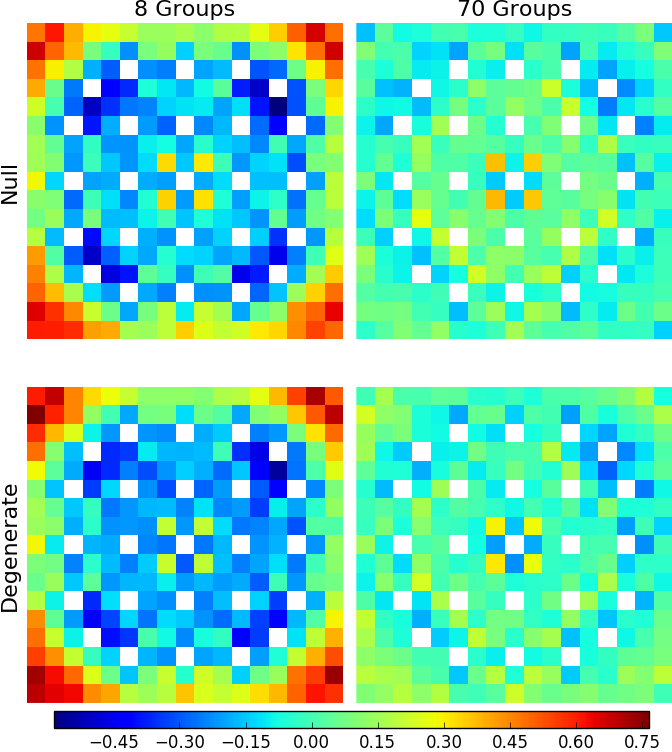
\includegraphics[width=\linewidth]{figures/quantification/assm-16/fiss-err}
\caption[Fission rate errors for a 1.6\% enriched assembly]{Fission rate errors for a 1.6\% enriched assembly.}
\label{fig:chap8-assm-1.6-fiss-err}
\end{figure}

\begin{figure}[h!]
\centering
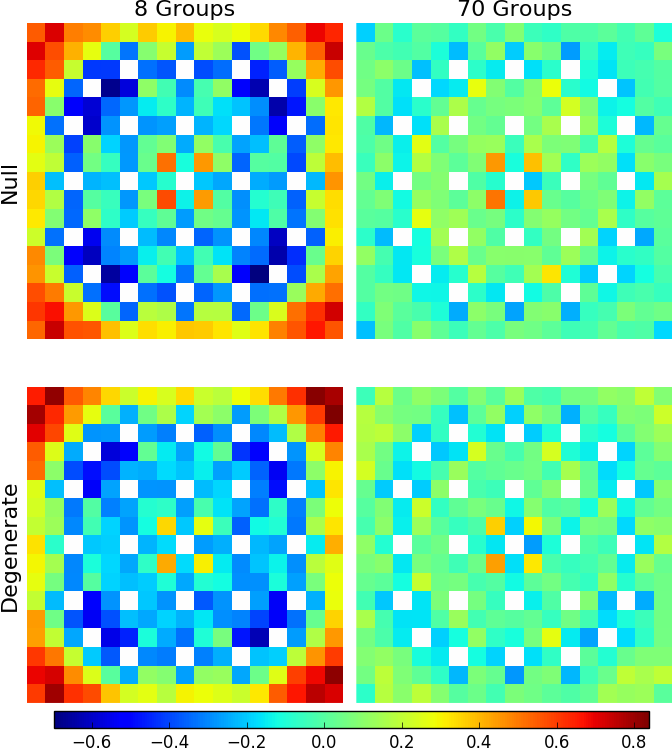
\includegraphics[width=\linewidth]{figures/quantification/assm-31/fiss-err}
\caption[Fission rate errors for a 3.1\% enriched assembly]{Fission rate errors for a 3.1\% enriched assembly.}
\label{fig:chap8-assm-3.1-fiss-err}
\end{figure}

\begin{figure}[h!]
\centering
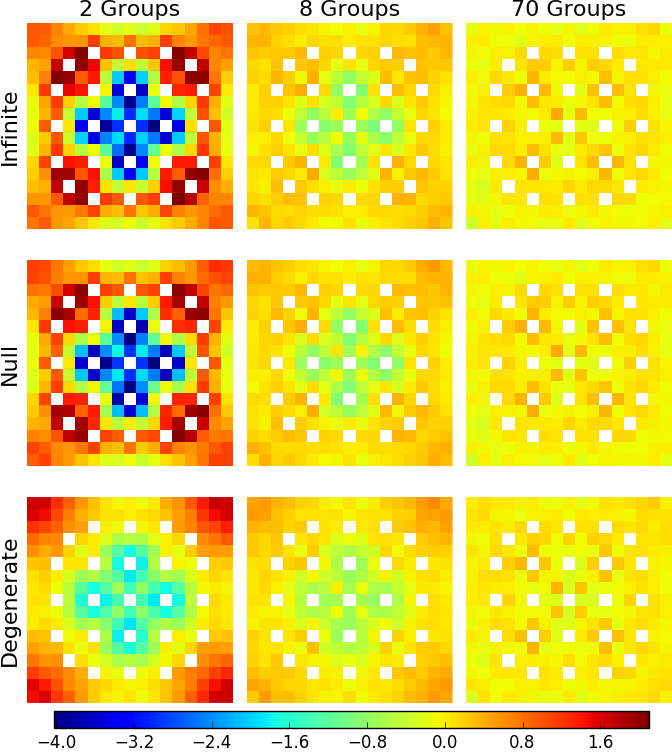
\includegraphics[width=\linewidth]{figures/quantification/assm-31-20BPs/fiss-err}
\caption[Fission rate errors for a 3.1\% enriched assembly with 20 BPs]{Fission rate errors for a 3.1\% enriched assembly with 20 BPs.}
\label{fig:chap8-assm-3.1-20BPs-fiss-err}
\end{figure}

\begin{figure}[h!]
\centering
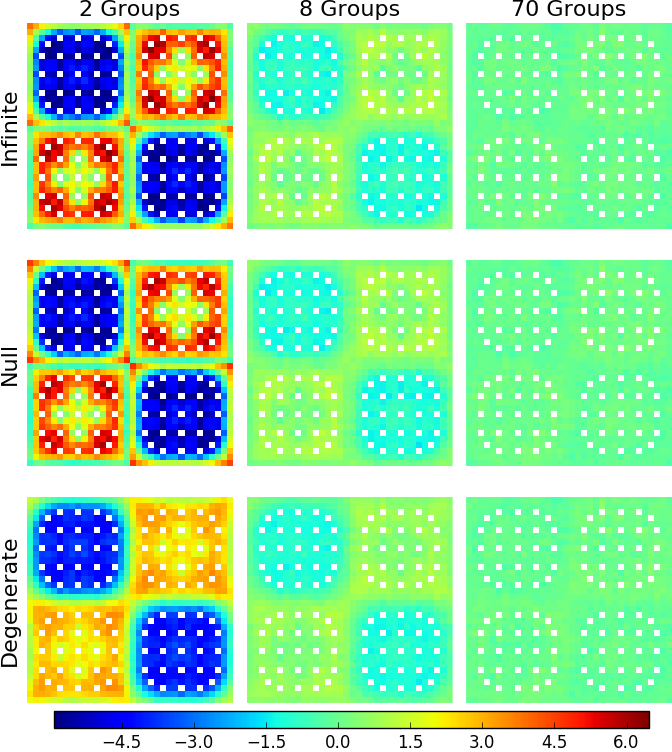
\includegraphics[width=\linewidth]{figures/quantification/2x2/fiss-err}
\caption[Fission rate errors for a 2$\times$2 colorset]{Fission rate errors for a 2$\times$2 colorset.}
\label{fig:chap8-2x2-fiss-err}
\end{figure}

\begin{figure}[h!]
\centering
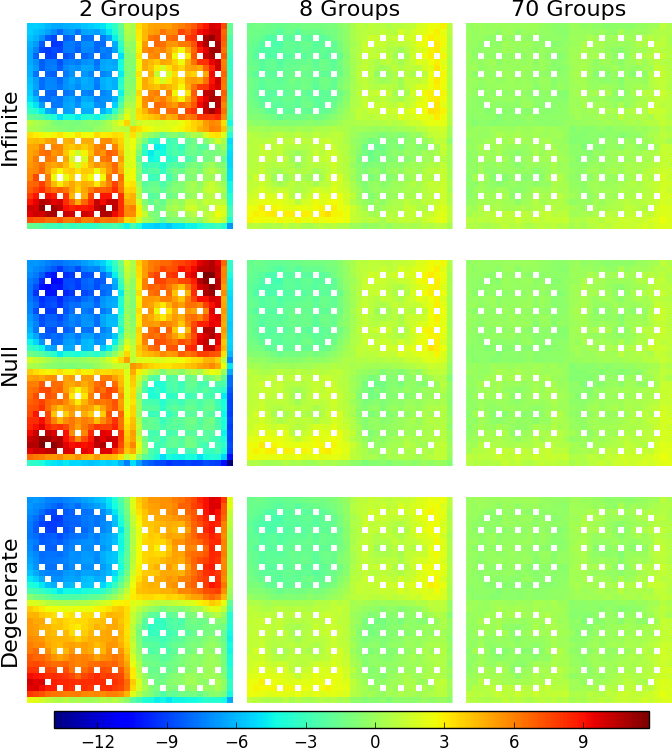
\includegraphics[width=\linewidth]{figures/quantification/reflector/fiss-err}
\caption[Fission rate errors for a 2$\times$2 colorset with a reflector]{Fission rate errors for a 2$\times$2 colorset with a reflector.}
\label{fig:chap8-reflector-fiss-err}
\end{figure}

\begin{figure}[h!]
\centering
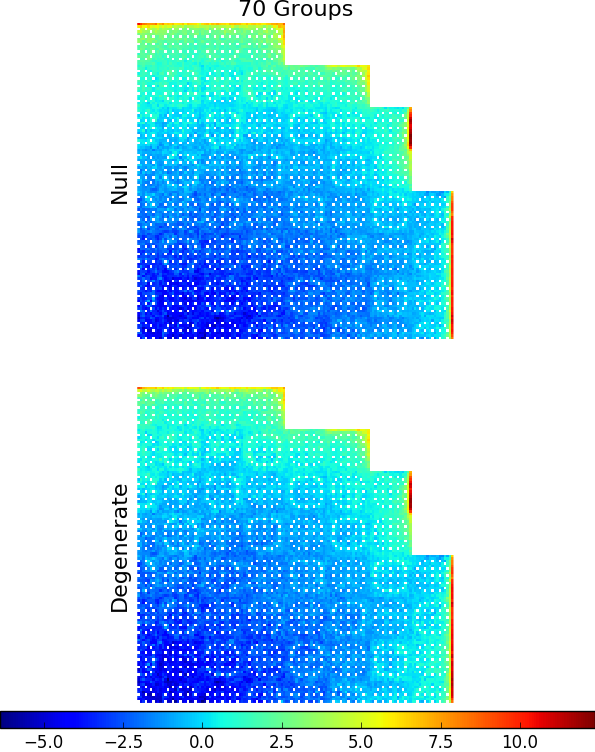
\includegraphics[width=\linewidth]{figures/quantification/full-core/fiss-err}
\caption[Fission rate errors for the 2D quarter core \ac{BEAVRS} model]{Fission rate errors for the 2D quarter core \ac{BEAVRS} model.}
\label{fig:chap8-full-core-fiss-err}
\end{figure}

\begin{itemize}[noitemsep]
  \item convergence rates for max/mean rel. err. for each benchmark
  \begin{itemize}[noitemsep]
    \item infinite vs. null vs. degenerate
    \item by energy group structure?
  \end{itemize}
  \item 2D heat maps of error distributions for each benchmark
  \begin{itemize}[noitemsep]
    \item infinite vs. null vs. degenerate
    \item by energy group structure?
  \end{itemize}
\end{itemize}

%%%%%%%%%%%%%%%%%%%%%%%%%%%%%%%%%%%%%%%%%%%%%
\subsection{U-238 Capture Rate Distributions}
\label{subsec:chap8-capt-rates}

\begin{table}[h!]
  \centering
  \caption[Maximum OpenMOC U-238 capture rate errors]{Maximum OpenMOC U-238 capture rate errors for varying spatial homogenization schemes and energy groups structures.}
  \small
  \label{table:chap8-openmoc-max-capt-rates}
  \vspace{6pt}
  \begin{tabular}{l l c c c}
  \toprule
  \rowcolor{lightgray}
  & & \multicolumn{3}{c}{\cellcolor{lightgray} \textbf{Max Error [\%]}} \\
  \multirow{-2}{*}{\cellcolor{lightgray} \bf Benchmark} &
  \multirow{-2}{*}{\cellcolor{lightgray} \bf \ac{MGXS} Scheme} &
  \multicolumn{1}{c}{{\cellcolor{lightgray} \bf 2-Group}} &
  \multicolumn{1}{c}{{\cellcolor{lightgray} \bf 8-Group}} &
  \multicolumn{1}{c}{{\cellcolor{lightgray} \bf 70-Group}} \\
  \midrule
\multirow{3}{*}{\parbox{2.5cm}{1.6\% Assm}} & Infinite & -2.86E+00 & -1.61E+00 & -1.17E+00 \\
& Null & -2.86E+00 & -1.60E+00 & -1.17E+00 \\
& Degenerate & 9.07E--01 & 3.88E--01 & 2.99E--01 \\
  \midrule
\multirow{3}{*}{\parbox{2.5cm}{3.1\% Assm}} & Infinite & -3.25E+00 & -1.91E+00 & -1.44E+00 \\
& Null & -3.24E+00 & -1.90E+00 & -1.44E+00 \\
& Degenerate & 8.14E--01 & 4.75E--01 & 3.39E--01 \\
  \midrule
\multirow{3}{*}{\parbox{2.5cm}{3.1\% Assm w/ 20 BPs}} & Infinite & 3.00E+00 & -1.30E+00 & -1.04E+00 \\
& Null & 3.02E+00 & -1.29E+00 & -1.04E+00 \\
& Degenerate & 1.36E+00 & 6.19E--01 & 2.96E--01 \\
  \midrule
\multirow{3}{*}{\parbox{2.5cm}{2$\times$2 Colorset}} & Infinite & -4.92E+00 & -2.09E+00 & -1.65E+00 \\
& Null & -4.52E+00 & -1.90E+00 & -1.59E+00 \\
& Degenerate & -2.12E+00 & -7.11E--01 & 4.75E--01 \\
  \midrule
\multirow{3}{*}{\parbox{2.5cm}{2$\times$2 Colorset w/ Reflector}} & Infinite & 1.27E+01 & 4.84E+00 & -2.42E+00 \\
& Null & 1.17E+01 & 3.74E+00 & -2.47E+00 \\
& Degenerate & 9.67E+00 & 3.28E+00 & -7.08E--01 \\
  \midrule
  \multirow{3}{*}{\parbox{2cm}{\ac{BEAVRS} Quarter Core}} & Infinite & 497 & 497 & \\
  & Null & & & \\
  & Degenerate & & & \\
  \bottomrule
\end{tabular}
\end{table}

\begin{table}[h!]
  \centering
  \caption[Mean OpenMOC U-238 capture rate errors]{Mean OpenMOC U-238 capture rate errors for varying spatial homogenization schemes and energy groups structures.}
  \small
  \label{table:chap8-openmoc-mean-capt-rates}
  \vspace{6pt}
  \begin{tabular}{l l c c c}
  \toprule
  \rowcolor{lightgray}
  & & \multicolumn{3}{c}{\cellcolor{lightgray} \textbf{Mean Error [\%]}} \\
  \multirow{-2}{*}{\cellcolor{lightgray} \bf Benchmark} &
  \multirow{-2}{*}{\cellcolor{lightgray} \bf \ac{MGXS} Scheme} &
  \multicolumn{1}{c}{{\cellcolor{lightgray} \bf 2-Group}} &
  \multicolumn{1}{c}{{\cellcolor{lightgray} \bf 8-Group}} &
  \multicolumn{1}{c}{{\cellcolor{lightgray} \bf 70-Group}} \\
  \midrule
\multirow{3}{*}{\parbox{2.5cm}{1.6\% Assm}} & Infinite & 3.41E--02 & 1.65E--02 & 1.17E--02 \\
& Null & 3.41E--02 & 1.65E--02 & 1.17E--02 \\
& Degenerate & 8.19E--03 & 5.01E--04 & 4.37E--04 \\
  \midrule
\multirow{3}{*}{\parbox{2.5cm}{3.1\% Assm}} & Infinite & 3.95E--02 & 1.98E--02 & 1.46E--02 \\
& Null & 3.94E--02 & 1.98E--02 & 1.46E--02 \\
& Degenerate & 8.15E--03 & -2.87E--04 & 4.77E--04 \\
  \midrule
\multirow{3}{*}{\parbox{2.5cm}{3.1\% Assm w/ 20 BPs}} & Infinite & -8.62E--03 & -3.80E--03 & -2.13E--03 \\
& Null & -7.91E--03 & -3.75E--03 & -2.17E--03 \\
& Degenerate & -3.50E--03 & -3.00E--03 & 2.29E--04 \\
  \midrule
\multirow{3}{*}{\parbox{2.5cm}{2$\times$2 Colorset}} & Infinite & 1.68E--01 & 1.71E--02 & 1.67E--02 \\
& Null & 1.28E--01 & 1.71E--03 & 1.13E--02 \\
& Degenerate & 9.91E--02 & -8.60E--03 & 6.92E--03 \\
  \midrule
\multirow{3}{*}{\parbox{2.5cm}{2$\times$2 Colorset w/ Reflector}} & Infinite & 1.90E+00 & 4.42E--01 & -2.59E--02 \\
& Null & 1.54E+00 & 3.60E--01 & -2.21E--02 \\
& Degenerate & 1.78E+00 & 4.42E--01 & 9.53E--03 \\
  \midrule
  \multirow{3}{*}{\parbox{2cm}{\ac{BEAVRS} Quarter Core}} & Infinite & 497 & 497 & \\
  & Null & & & \\
  & Degenerate & & & \\
  \bottomrule
\end{tabular}
\end{table}


\begin{figure}[h!]
\centering
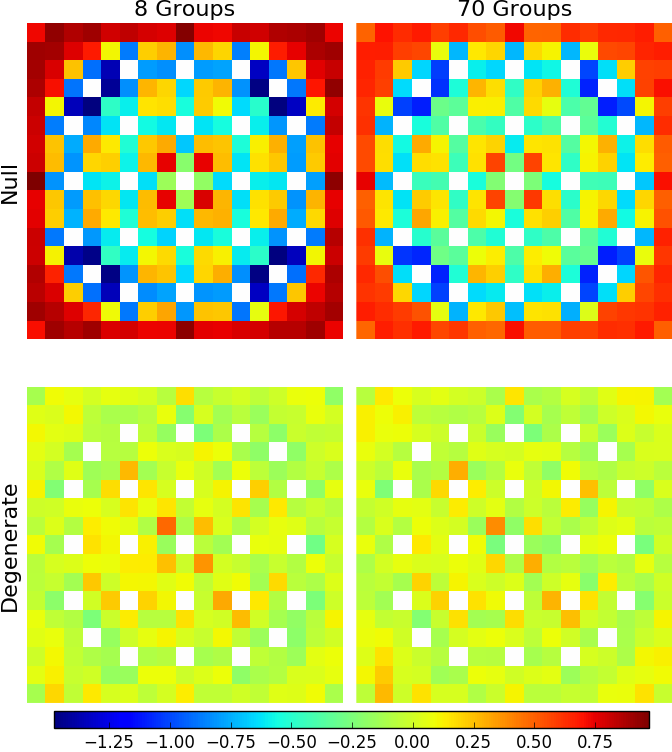
\includegraphics[width=\linewidth]{figures/quantification/assm-16/capt-err}
\caption[U-238 capture rate errors for a 1.6\% enriched assembly]{U-238 capture rate errors for a 1.6\% enriched assembly.}
\label{fig:chap8-assm-1.6-capt-err}
\end{figure}

\begin{figure}[h!]
\centering
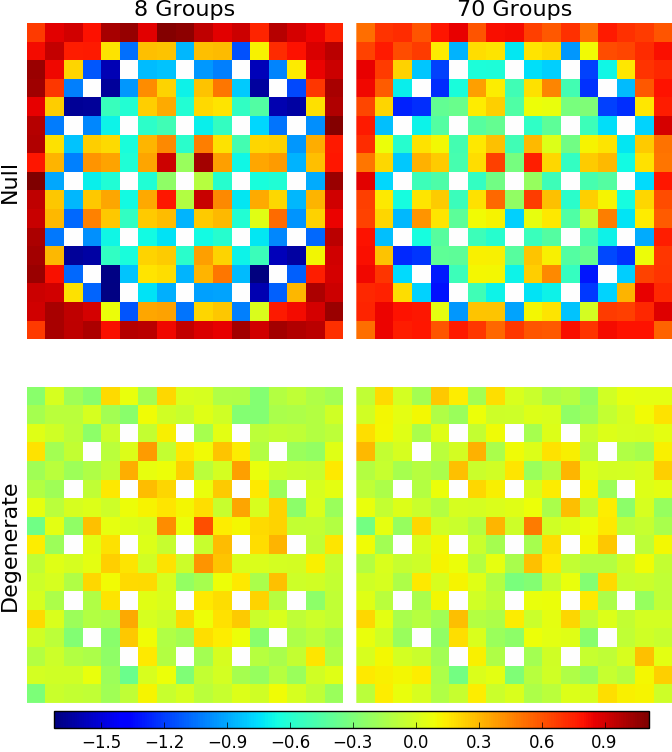
\includegraphics[width=\linewidth]{figures/quantification/assm-31/capt-err}
\caption[U-238 capture rate errors for a 3.1\% enriched assembly]{U-238 capture rate errors for a 3.1\% enriched assembly.}
\label{fig:chap8-assm-3.1-capt-err}
\end{figure}

\begin{figure}[h!]
\centering
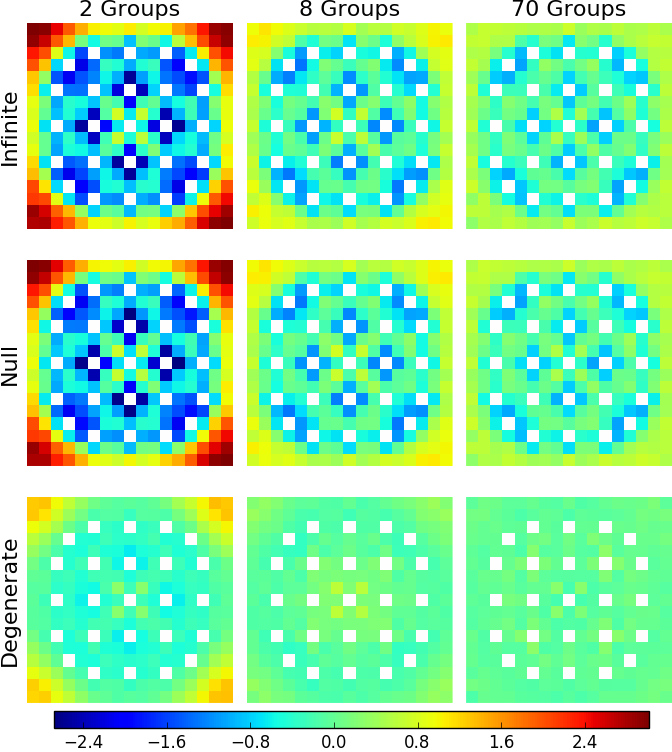
\includegraphics[width=\linewidth]{figures/quantification/assm-31-20BPs/capt-err}
\caption[U-238 capture rate errors for a 3.1\% enriched assembly with 20 BPs]{U-238 capture rate errors for a 3.1\% enriched assembly with 20 BPs.}
\label{fig:chap8-assm-3.1-20BPs-capt-err}
\end{figure}

\begin{figure}[h!]
\centering
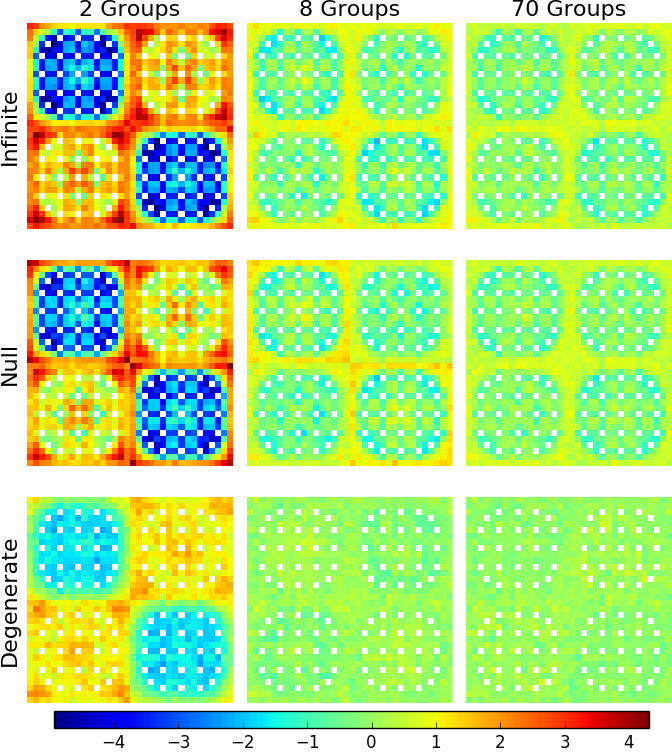
\includegraphics[width=\linewidth]{figures/quantification/2x2/capt-err}
\caption[U-238 capture rate errors for a 2$\times$2 colorset]{U-238 capture rate errors for a 2$\times$2 colorset.}
\label{fig:chap8-2x2-capt-err}
\end{figure}

\begin{figure}[h!]
\centering
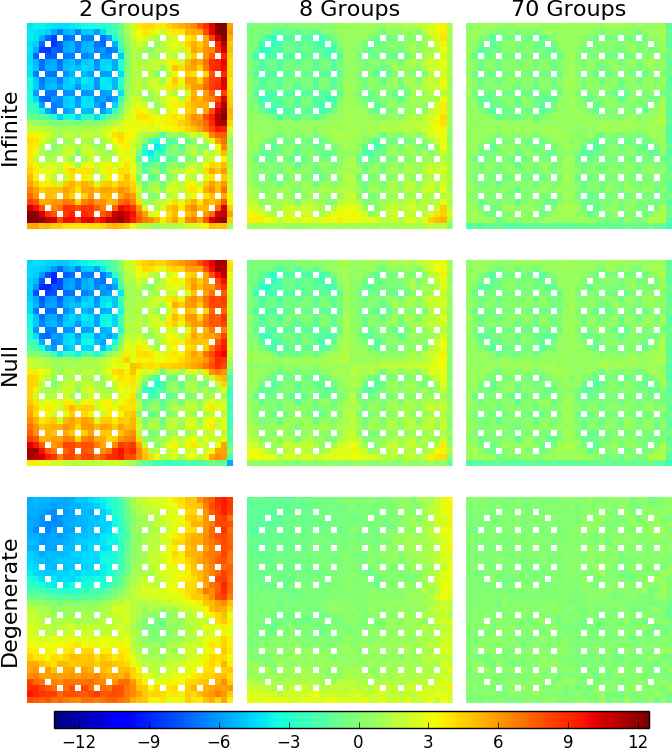
\includegraphics[width=\linewidth]{figures/quantification/reflector/capt-err}
\caption[U-238 capture rate errors for a 2$\times$2 colorset with a reflector]{U-238 capture rate errors for a 2$\times$2 colorset with a reflector.}
\label{fig:chap8-reflector-capt-err}
\end{figure}

\begin{figure}[h!]
\centering
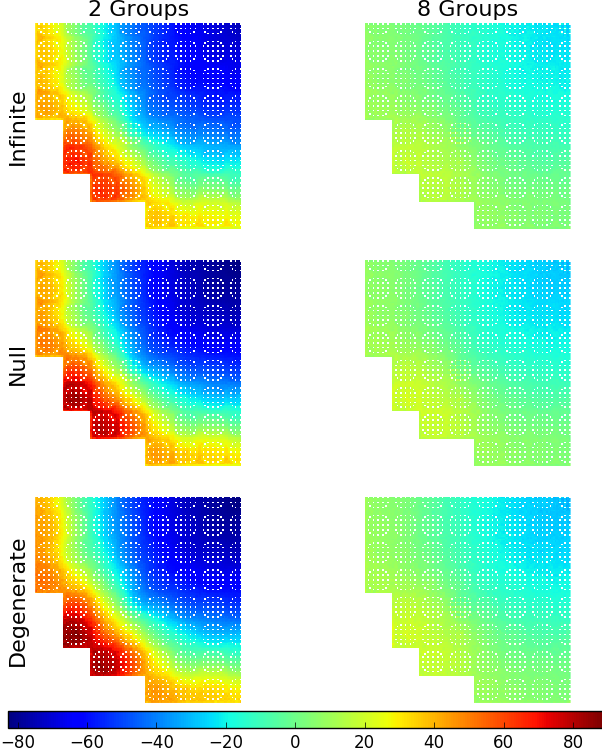
\includegraphics[width=\linewidth]{figures/quantification/full-core/capt-err}
\caption[U-238 capture rate errors for the 2D quarter core \ac{BEAVRS} model]{U-238 capture rate errors for the 2D quarter core \ac{BEAVRS} model.}
\label{fig:chap8-full-core-capt-err}
\end{figure}


\begin{itemize}[noitemsep]
  \item convergence rates for max/mean rel. err. for each benchmark
  \begin{itemize}[noitemsep]
    \item infinite vs. null vs. degenerate
    \item by energy group structure?
  \end{itemize}
  \item 2D heat maps of error distributions for each benchmark
  \begin{itemize}[noitemsep]
    \item infinite vs. null vs. degenerate
    \item by energy group structure?
  \end{itemize}
\end{itemize}


%%%%%%%%%%%%%%%%%%%%%%%%%%%%%%%%%%%%%%%%%%%%%%%%%%%%%%%%%%%%%%%%%%%%%%%%%%%%%%%
\section{MGXS Convergence Rates}
\label{sec:chap8-mgxs-converge}

\begin{itemize}[noitemsep]
  \item Plot evolution of rel. err. by batch for each homogenization scheme
  \begin{itemize}[noitemsep]
    \item groups with highest rel. err.
    \item reactions with greatest contribution to eigenvalue (U-238 capture)
    \item total (track-length) vs. scattering matrices (analog)    
    \item which group structure(s)?
 \end{itemize}
  \item compare to pin power convergence rates in preceding chapter
\end{itemize}

%-infinite vs. null vs. degenerate
%-conv rates for MGXS in each case - choose worst groups
%  -compare back to pin power error conv. rates
%  -convergence rates for infinite vs. null vs. degenerate